\documentclass[sigconf,edbt]{acmart-edbt2025}

\def\BibTeX{{\rm B\kern-.05em{\sc i\kern-.025em b}\kern-.08em
    T\kern-.1667em\lower.7ex\hbox{E}\kern-.125emX}}


%\usepackage{amsmath,amssymb,amsfonts}
%$\mathbb{k}$
\usepackage{booktabs} % For formal tables
\usepackage{algorithm}
\usepackage{algorithmic}
\usepackage{graphicx}
\usepackage{textcomp}
\usepackage{multirow}
\usepackage{hyperref} % 引入 hyperref 宏包
\usepackage{enumitem} %用于item空白对其
\usepackage{makecell} % Allows for line breaks within table cells
\usepackage{tabularx}
\usepackage{tcolorbox}
\usepackage{wrapfig}  % 引入 wrapfig 包实现文字环绕
%\usepackage{lmodern}
\usepackage[T1]{fontenc}


% Copyright
\setcopyright{rightsretained}

% DOI
\acmDOI{}

% ISBN
\acmISBN{978-3-89318-099-8}

%Conference
\acmConference[EDBT 2025]{28th International Conference on Extending Database Technology (EDBT)}{25th March-28th March, 2025}{Barcelona, Spain}
\acmYear{2025}

\settopmatter{printacmref=false, printccs=false, printfolios=false}

\pagestyle{empty} % removes running headers


\begin{document}
\title{Automated Data Quality Validation in an End-to-End GNN Framework}
%\titlenote{Produces the permission block, and copyright information}
% \subtitle{Extended Abstract}
% \subtitlenote{The full version of the author's guide is available as
%   \texttt{acmart.pdf} document}
  

% themis red comment
\newcommand{\tp}[1]{{\color{red} {\bf ??? #1 ???}}\normalcolor}
\newcommand{\qw}[1]{{\color{red} {\bf (qitong: #1)}}\normalcolor}
\newcommand{\sijie}[1]{{\color{blue} {\bf (sijie: #1)   }}\normalcolor}
\newcommand{\sj}[1]{{\color{red} {#1}}\normalcolor}
\newcommand{\soror}[1]{{\color{violet} {\bf (soror: #1)   }}\normalcolor}



\author{Sijie Dong}
\affiliation{%
  \institution{Université Paris Cité}
  \streetaddress{}
  \city{Paris}
  \country{France}
}
\email{sijie.dong@etu.u-paris.fr}

\author{Soror Sahri}
\affiliation{%
  \institution{Université Paris Cité}
  \city{Paris}
  \country{France}
}
\email{soror.sahri@parisdescartes.fr}

\author{Themis Palpanas}
\affiliation{%
  \institution{Université Paris Cité}
  \city{Paris}
  \country{France}
}
\email{themis@mi.parisdescartes.fr}

\author{Qitong Wang}
\affiliation{%
  \institution{Harvard University}
  \streetaddress{}
  \city{Boston}
  \country{USA}
}
\email{qitong@seas.harvard.edu}

% The default list of authors is too long for headers}
% \renewcommand{\shortauthors}{B. Trovato et al.}
\renewcommand{\shortauthors}{}


\begin{abstract}
Ensuring data quality is crucial in modern data ecosystems, especially for training or testing datasets in machine learning. 
Existing validation approaches rely on computing data quality metrics and/or using expert-defined constraints. 
Although there are automated constraint generation methods, they are often incomplete and may be too strict or too soft, causing false positives or missed errors, thus requiring expert adjustment. 
These methods may also fail to detect subtle data inconsistencies hidden by complex interdependencies within the data.
In this paper, we propose DQuag, an end-to-end data quality validation and repair framework based on an improved Graph Neural Network (GNN) and multi-task learning. The proposed method incorporates a dual-decoder design: one for data quality validation and the other for data repair.
Our approach captures complex feature relationships within tabular datasets using a multi-layer GNN architecture 
%that combines Graph Attention Networks (GAT) and Graph Isomorphism Networks (GIN) 
to automatically detect explicit and hidden data errors. 
Unlike previous methods, our model does not require manual input for constraint generation and learns the underlying feature dependencies, enabling it to identify complex hidden errors that traditional systems often miss. 
Moreover, it can recommend repair values, improving overall data quality. 
Experimental results validate the effectiveness of our approach in identifying and resolving data quality issues. The paper appeared in EDBT 2025.
\end{abstract}

%
% % The code below should be generated by the tool at
% % http://dl.acm.org/ccs.cfm
% % Please copy and paste the code instead of the example below. 
% %
% \begin{CCSXML}
% <ccs2012>
%  <concept>
%   <concept_id>10010520.10010553.10010562</concept_id>
%   <concept_desc>Computer systems organization~Embedded systems</concept_desc>
%   <concept_significance>500</concept_significance>
%  </concept>
%  <concept>
%   <concept_id>10010520.10010575.10010755</concept_id>
%   <concept_desc>Computer systems organization~Redundancy</concept_desc>
%   <concept_significance>300</concept_significance>
%  </concept>
%  <concept>
%   <concept_id>10010520.10010553.10010554</concept_id>
%   <concept_desc>Computer systems organization~Robotics</concept_desc>
%   <concept_significance>100</concept_significance>
%  </concept>
%  <concept>
%   <concept_id>10003033.10003083.10003095</concept_id>
%   <concept_desc>Networks~Network reliability</concept_desc>
%   <concept_significance>100</concept_significance>
%  </concept>
% </ccs2012>  
% \end{CCSXML}
% 
% \ccsdesc[500]{Computer systems organization~Embedded systems}
% \ccsdesc[300]{Computer systems organization~Redundancy}
% \ccsdesc{Computer systems organization~Robotics}
% \ccsdesc[100]{Networks~Network reliability}


% \keywords{ACM proceedings, \LaTeX, text tagging}

%% A "teaser" image appears between the author and affiliation
%% information and the body of the document, and typically spans the
%% page.
% \begin{teaserfigure}
%   \includegraphics[width=\textwidth]{sampleteaser}
%   \caption{Seattle Mariners at Spring Training, 2010.}
%   \label{fig:teaser}
% \end{teaserfigure}

\maketitle

\section{Introduction}
\label{sec:introduction}
The business processes of organizations are experiencing ever-increasing complexity due to the large amount of data, high number of users, and high-tech devices involved \cite{martin2021pmopportunitieschallenges, beerepoot2023biggestbpmproblems}. This complexity may cause business processes to deviate from normal control flow due to unforeseen and disruptive anomalies \cite{adams2023proceddsriftdetection}. These control-flow anomalies manifest as unknown, skipped, and wrongly-ordered activities in the traces of event logs monitored from the execution of business processes \cite{ko2023adsystematicreview}. For the sake of clarity, let us consider an illustrative example of such anomalies. Figure \ref{FP_ANOMALIES} shows a so-called event log footprint, which captures the control flow relations of four activities of a hypothetical event log. In particular, this footprint captures the control-flow relations between activities \texttt{a}, \texttt{b}, \texttt{c} and \texttt{d}. These are the causal ($\rightarrow$) relation, concurrent ($\parallel$) relation, and other ($\#$) relations such as exclusivity or non-local dependency \cite{aalst2022pmhandbook}. In addition, on the right are six traces, of which five exhibit skipped, wrongly-ordered and unknown control-flow anomalies. For example, $\langle$\texttt{a b d}$\rangle$ has a skipped activity, which is \texttt{c}. Because of this skipped activity, the control-flow relation \texttt{b}$\,\#\,$\texttt{d} is violated, since \texttt{d} directly follows \texttt{b} in the anomalous trace.
\begin{figure}[!t]
\centering
\includegraphics[width=0.9\columnwidth]{images/FP_ANOMALIES.png}
\caption{An example event log footprint with six traces, of which five exhibit control-flow anomalies.}
\label{FP_ANOMALIES}
\end{figure}

\subsection{Control-flow anomaly detection}
Control-flow anomaly detection techniques aim to characterize the normal control flow from event logs and verify whether these deviations occur in new event logs \cite{ko2023adsystematicreview}. To develop control-flow anomaly detection techniques, \revision{process mining} has seen widespread adoption owing to process discovery and \revision{conformance checking}. On the one hand, process discovery is a set of algorithms that encode control-flow relations as a set of model elements and constraints according to a given modeling formalism \cite{aalst2022pmhandbook}; hereafter, we refer to the Petri net, a widespread modeling formalism. On the other hand, \revision{conformance checking} is an explainable set of algorithms that allows linking any deviations with the reference Petri net and providing the fitness measure, namely a measure of how much the Petri net fits the new event log \cite{aalst2022pmhandbook}. Many control-flow anomaly detection techniques based on \revision{conformance checking} (hereafter, \revision{conformance checking}-based techniques) use the fitness measure to determine whether an event log is anomalous \cite{bezerra2009pmad, bezerra2013adlogspais, myers2018icsadpm, pecchia2020applicationfailuresanalysispm}. 

The scientific literature also includes many \revision{conformance checking}-independent techniques for control-flow anomaly detection that combine specific types of trace encodings with machine/deep learning \cite{ko2023adsystematicreview, tavares2023pmtraceencoding}. Whereas these techniques are very effective, their explainability is challenging due to both the type of trace encoding employed and the machine/deep learning model used \cite{rawal2022trustworthyaiadvances,li2023explainablead}. Hence, in the following, we focus on the shortcomings of \revision{conformance checking}-based techniques to investigate whether it is possible to support the development of competitive control-flow anomaly detection techniques while maintaining the explainable nature of \revision{conformance checking}.
\begin{figure}[!t]
\centering
\includegraphics[width=\columnwidth]{images/HIGH_LEVEL_VIEW.png}
\caption{A high-level view of the proposed framework for combining \revision{process mining}-based feature extraction with dimensionality reduction for control-flow anomaly detection.}
\label{HIGH_LEVEL_VIEW}
\end{figure}

\subsection{Shortcomings of \revision{conformance checking}-based techniques}
Unfortunately, the detection effectiveness of \revision{conformance checking}-based techniques is affected by noisy data and low-quality Petri nets, which may be due to human errors in the modeling process or representational bias of process discovery algorithms \cite{bezerra2013adlogspais, pecchia2020applicationfailuresanalysispm, aalst2016pm}. Specifically, on the one hand, noisy data may introduce infrequent and deceptive control-flow relations that may result in inconsistent fitness measures, whereas, on the other hand, checking event logs against a low-quality Petri net could lead to an unreliable distribution of fitness measures. Nonetheless, such Petri nets can still be used as references to obtain insightful information for \revision{process mining}-based feature extraction, supporting the development of competitive and explainable \revision{conformance checking}-based techniques for control-flow anomaly detection despite the problems above. For example, a few works outline that token-based \revision{conformance checking} can be used for \revision{process mining}-based feature extraction to build tabular data and develop effective \revision{conformance checking}-based techniques for control-flow anomaly detection \cite{singh2022lapmsh, debenedictis2023dtadiiot}. However, to the best of our knowledge, the scientific literature lacks a structured proposal for \revision{process mining}-based feature extraction using the state-of-the-art \revision{conformance checking} variant, namely alignment-based \revision{conformance checking}.

\subsection{Contributions}
We propose a novel \revision{process mining}-based feature extraction approach with alignment-based \revision{conformance checking}. This variant aligns the deviating control flow with a reference Petri net; the resulting alignment can be inspected to extract additional statistics such as the number of times a given activity caused mismatches \cite{aalst2022pmhandbook}. We integrate this approach into a flexible and explainable framework for developing techniques for control-flow anomaly detection. The framework combines \revision{process mining}-based feature extraction and dimensionality reduction to handle high-dimensional feature sets, achieve detection effectiveness, and support explainability. Notably, in addition to our proposed \revision{process mining}-based feature extraction approach, the framework allows employing other approaches, enabling a fair comparison of multiple \revision{conformance checking}-based and \revision{conformance checking}-independent techniques for control-flow anomaly detection. Figure \ref{HIGH_LEVEL_VIEW} shows a high-level view of the framework. Business processes are monitored, and event logs obtained from the database of information systems. Subsequently, \revision{process mining}-based feature extraction is applied to these event logs and tabular data input to dimensionality reduction to identify control-flow anomalies. We apply several \revision{conformance checking}-based and \revision{conformance checking}-independent framework techniques to publicly available datasets, simulated data of a case study from railways, and real-world data of a case study from healthcare. We show that the framework techniques implementing our approach outperform the baseline \revision{conformance checking}-based techniques while maintaining the explainable nature of \revision{conformance checking}.

In summary, the contributions of this paper are as follows.
\begin{itemize}
    \item{
        A novel \revision{process mining}-based feature extraction approach to support the development of competitive and explainable \revision{conformance checking}-based techniques for control-flow anomaly detection.
    }
    \item{
        A flexible and explainable framework for developing techniques for control-flow anomaly detection using \revision{process mining}-based feature extraction and dimensionality reduction.
    }
    \item{
        Application to synthetic and real-world datasets of several \revision{conformance checking}-based and \revision{conformance checking}-independent framework techniques, evaluating their detection effectiveness and explainability.
    }
\end{itemize}

The rest of the paper is organized as follows.
\begin{itemize}
    \item Section \ref{sec:related_work} reviews the existing techniques for control-flow anomaly detection, categorizing them into \revision{conformance checking}-based and \revision{conformance checking}-independent techniques.
    \item Section \ref{sec:abccfe} provides the preliminaries of \revision{process mining} to establish the notation used throughout the paper, and delves into the details of the proposed \revision{process mining}-based feature extraction approach with alignment-based \revision{conformance checking}.
    \item Section \ref{sec:framework} describes the framework for developing \revision{conformance checking}-based and \revision{conformance checking}-independent techniques for control-flow anomaly detection that combine \revision{process mining}-based feature extraction and dimensionality reduction.
    \item Section \ref{sec:evaluation} presents the experiments conducted with multiple framework and baseline techniques using data from publicly available datasets and case studies.
    \item Section \ref{sec:conclusions} draws the conclusions and presents future work.
\end{itemize}
\section{Related Work}
The landscape of large language model vulnerabilities has been extensively studied in recent literature \cite{crothers2023machinegeneratedtextcomprehensive,shayegani2023surveyvulnerabilitieslargelanguage,Yao_2024,Huang2023ASO}, that propose detailed taxonomies of threats. These works categorize LLM attacks into distinct types, such as adversarial attacks, data poisoning, and specific vulnerabilities related to prompt engineering. Among these, prompt injection attacks have emerged as a significant and distinct category, underscoring their relevance to LLM security.

The following high-level overview of the collected taxonomy of LLM vulnerabilities is defined in \cite{Yao_2024}:
\begin{itemize}
    \item Adversarial Attacks: Data Poisoning, Backdoor Attacks
    \item Inference Attacks: Attribute Inference, Membership Inferences
    \item Extraction Attacks
    \item Bias and Unfairness
Exploitation
    \item Instruction Tuning Attacks: Jailbreaking, Prompt Injection.
\end{itemize}
Prompt injection attacks are further classified in \cite{shayegani2023surveyvulnerabilitieslargelanguage} into the following: Goal hijacking and \textbf{Prompt leakage}.

The reviewed taxonomies underscore the need for comprehensive frameworks to evaluate LLM security. The agentic approach introduced in this paper builds on these insights, automating adversarial testing to address a wide range of scenarios, including those involving prompt leakage and role-specific vulnerabilities.

\subsection{Prompt Injection and Prompt Leakage}

Prompt injection attacks exploit the blending of instructional and data inputs, manipulating LLMs into deviating from their intended behavior. Prompt injection attacks encompass techniques that override initial instructions, expose private prompts, or generate malicious outputs \cite{Huang2023ASO}. A subset of these attacks, known as prompt leakage, aims specifically at extracting sensitive system prompts embedded within LLM configurations. In \cite{shayegani2023surveyvulnerabilitieslargelanguage}, authors differentiate between prompt leakage and related methods such as goal hijacking, further refining the taxonomy of LLM-specific vulnerabilities.

\subsection{Defense Mechanisms}

Various defense mechanisms have been proposed to address LLM vulnerabilities, particularly prompt injection and leakage \cite{shayegani2023surveyvulnerabilitieslargelanguage,Yao_2024}. We focused on cost-effective methods like instruction postprocessing and prompt engineering, which are viable for proprietary models that cannot be retrained. Instruction preprocessing sanitizes inputs, while postprocessing removes harmful outputs, forming a dual-layer defense. Preprocessing methods include perplexity-based filtering \cite{Jain2023BaselineDF,Xu2022ExploringTU} and token-level analysis \cite{Kumar2023CertifyingLS}. Postprocessing employs another set of techniques, such as censorship by LLMs \cite{Helbling2023LLMSD,Inan2023LlamaGL}, and use of canary tokens and pattern matching \cite{vigil-llm,rebuff}, although their fundamental limitations are noted \cite{Glukhov2023LLMCA}. Prompt engineering employs carefully designed instructions \cite{Schulhoff2024ThePR} and advanced techniques like spotlighting \cite{Hines2024DefendingAI} to mitigate vulnerabilities, though no method is foolproof \cite{schulhoff-etal-2023-ignore}. Adversarial training, by incorporating adversarial examples into the training process, strengthens models against attacks \cite{Bespalov2024TowardsBA,Shaham2015UnderstandingAT}.

\subsection{Security Testing for Prompt Injection Attacks}

Manual testing, such as red teaming \cite{ganguli2022redteaminglanguagemodels} and handcrafted "Ignore Previous Prompt" attacks \cite{Perez2022IgnorePP}, highlights vulnerabilities but is limited in scale. Automated approaches like PAIR \cite{chao2024jailbreakingblackboxlarge} and GPTFUZZER \cite{Yu2023GPTFUZZERRT} achieve higher success rates by refining prompts iteratively or via automated fuzzing. Red teaming with LLMs \cite{Perez2022RedTL} and reinforcement learning \cite{anonymous2024diverse} uncovers diverse vulnerabilities, including data leakage and offensive outputs. Indirect Prompt Injection (IPI) manipulates external data to compromise applications \cite{Greshake2023NotWY}, adapting techniques like SQL injection to LLMs \cite{Liu2023PromptIA}. Prompt secrecy remains fragile, with studies showing reliable prompt extraction \cite{Zhang2023EffectivePE}. Advanced frameworks like Token Space Projection \cite{Maus2023AdversarialPF} and Weak-to-Strong Jailbreaking Attacks \cite{zhao2024weaktostrongjailbreakinglargelanguage} exploit token-space relationships, achieving high success rates for prompt extraction and jailbreaking.

\subsection{Agentic Frameworks for Evaluating LLM Security}

The development of multi-agent systems leveraging large language models (LLMs) has shown promising results in enhancing task-solving capabilities \cite{Hong2023MetaGPTMP, Wang2023UnleashingTE, Talebirad2023MultiAgentCH, Wu2023AutoGenEN, Du2023ImprovingFA}. A key aspect across various frameworks is the specialization of roles among agents \cite{Hong2023MetaGPTMP, Wu2023AutoGenEN}, which mimics human collaboration and improves task decomposition.

Agentic frameworks and the multi-agent debate approach benefit from agent interaction, where agents engage in conversations or debates to refine outputs and correct errors \cite{Wu2023AutoGenEN}. For example, debate systems improve factual accuracy and reasoning by iteratively refining responses through collaborative reasoning \cite{Du2023ImprovingFA}, while AG2 allows agents to autonomously interact and execute tasks with minimal human input.

These frameworks highlight the viability of agentic systems, showing how specialized roles and collaborative mechanisms lead to improved performance, whether in factuality, reasoning, or task execution. By leveraging the strengths of diverse agents, these systems demonstrate a scalable approach to problem-solving.

Recent research on testing LLMs using other LLMs has shown that this approach can be highly effective \cite{chao2024jailbreakingblackboxlarge, Yu2023GPTFUZZERRT, Perez2022RedTL}. Although the papers do not explicitly employ agentic frameworks they inherently reflect a pattern similar to that of an "attacker" and a "judge". \cite{chao2024jailbreakingblackboxlarge}  This pattern became a focal point for our work, where we put the judge into a more direct dialogue, enabling it to generate attacks based on the tested agent response in an active conversation.

A particularly influential paper in shaping our approach is Jailbreaking Black Box Large Language Models in Twenty Queries \cite{chao2024jailbreakingblackboxlarge}. This paper not only introduced the attacker/judge architecture but also provided the initial system prompts used for a judge.
\section{OUR APPROACH: DQuaG}

\begin{figure*}[tb]
\centering
\includegraphics[width=0.7\textwidth]{Figures/structure.pdf}
%\vspace{-0.6\baselineskip}
\caption{Data Quality Validation Framework Using GNN. Top: Training on clean data. Bottom: Validating unseen data by reconstruction error comparison.}
%\vspace*{-0.3cm}
%\soror{highlight in the caption the process at the top and the one at the bottom of teh figure }
\label{fig:framework}
\end{figure*}

%In this section, we detail our novel approach to automated data quality validation using graph representation learning and a Variational Autoencoder (VAE) framework. Assuming we start with a clean dataset, our method addresses the limitations of traditional data quality verification techniques through a series of steps designed to capture intrinsic relationships within tabular data and assess data quality with minimal expert intervention.


In this section, we present DQuaG (Data Quality Graph), a novel approach for data quality validation. 
Figure~\ref{fig:framework} illustrates the framework of our approach, which includes two main phases: model training on a clean dataset and data quality validation and repair for new data. 
In Phase 1, we train a model using a clean dataset to learn the normal patterns and relationships between features. 
In Phase 2, we use the trained model to assess the quality of new data and provide repair suggestions for any detected errors. 
%Our method incorporates several key innovations, including the use of an improved Graph Neural Network (GNN) encoder combining Graph Attention Network (GAT) and Graph Isomorphism Network (GIN), and a multi-task learning framework with dual decoders for data quality validation and repair. 


\subsection{Phase 1: Training GNN on Clean Data}
%\soror{it's betetr to remove data preprocessing as a step as we don't see it in the figure! we can only keep its text}
%\subsubsection{\textbf{Data Preprocessing}}
We assume the availability of a high-quality, clean dataset, $\mathcal{D}_{\text{clean}}$, that has undergone rigorous quality control and is free from errors. This dataset serves as the foundation for training our model. 
For feature encoding and normalization, categorical features are converted to numerical form using label encoding, where the encoder is fitted on both clean data and any possible future data to ensure consistency. 
For numerical features, we apply min-max normalization to scale values to the range [0, 1], which helps improve training stability and ensures that all features are on a comparable scale.


\subsubsection{\textbf{Feature Graph Construction}}

We use ChatGPT-4~\cite{openai2024gpt4} to automate the feature graph construction. 
Given a clean dataset, we extract the feature names ($F$) and their descriptions ($D$) from the data source. We then randomly sample 100 data points from the dataset, denoted as ($S$). 
These feature names, descriptions, and sample points are provided to ChatGPT-4 in a structured format to infer potential relationships between features. 
The output from ChatGPT-4 is a JSON file capturing feature relationships, which we denote as  \(\text{Feature\_Relationships} = \{ (f_i, f_j) \mid f_i, f_j \in F \}\), indicating that there is a relationship between features \( f_i \) and \( f_j \).

%The prompt used for ChatGPT-4 is as follows:
\begin{tcolorbox}[
    sharp corners=south,
    colback=white!98!black,
    colframe=white!45!black,
    boxrule=0.5mm,
    width=0.48\textwidth,
    enlarge left by=0mm,
    enlarge right by=0mm,
    arc=5mm,
    outer arc=3mm,
    %drop shadow south east={shadow xshift=0.5ex, shadow yshift=-0.5ex, fill=black!20},
    fonttitle=\bfseries,
    title=Prompt for Feature Relationship Inference,
    before upper=\par\small,
    after upper=\par\small
]
\vspace*{-0.2cm}
\small
Given the following information, please infer the relationships between features. Provide your output in JSON format, capturing the type of relationships.\newline
\textbf{Feature Names:} {List of feature names ($F$)}\newline
\textbf{Feature Descriptions:} {List of descriptions ($D$) for each feature}\newline
\textbf{Sample Data Points:} {100 data samples ($S$) from the dataset}\newline
\textbf{Output:} Please return a JSON object in the format:
\begin{verbatim}
{"relationships": [{"feature1", "feature2"}, 
                   {"feature3", "feature4"}, ...]}
\end{verbatim}
\vspace*{-0.3cm}
\end{tcolorbox}




Using these relationships, we construct the knowledge-based feature graph \( G = (V, E) \), where \( V \) represents features and \( E \) represents edges indicating relationships between features.

% \subsubsection{\textbf{Feature Graph Construction}}

% The initial step in our approach involves constructing a feature graph from clean tabular data to capture intrinsic relationships and dependencies between data features.
% First, we address the challenge of diverse data types: categorical variables are transformed using label encoding, and timestamp data is broken into components (i.e., day, month, year). 
% This uniform input format is critical for graph-based processing.

% We use ChatGPT-4~\cite{openai2024gpt4} to automate the feature graph construction. 
% Given a clean dataset, we extract the feature names \( F \) and their descriptions \( D \) from the data source. We then randomly sample 100 data points from the dataset, denoted as \( S \). These feature names, descriptions, and sample data points are provided to the ChatGPT-4, structured as follows: \(\text{Input} = \{ F, D, S \}\), then ChatGPT-4 generates a JSON file capturing feature relationships.
% The output format is \(\text{Feature\_Relationships} = \{ (f_i, f_j) \mid f_i, f_j \in F \}\), indicating that there is a relationship between features \( f_i \) and \( f_j \).

% Using these relationships, we construct the knowledge-based feature graph \( G = (V, E) \), where \( V \) represents features and \( E \) represents edges indicating relationships between features.

% \subsubsection{\textbf{Feature Graph Construction}}

% The initial step in our methodology involves constructing a feature graph from clean tabular data, which is essential for capturing the intrinsic relationships and dependencies between different data features.

% To facilitate this process, our approach first addresses the challenge of handling diverse data types. 
% In the preprocessing stage, categorical variables are transformed using label encoding, which assigns each unique category a unique integer based on alphabetical ordering. 
% For timestamp data, we extract significant components such as day, month, and year. 
% This uniform input format is critical for the subsequent graph-based processing. 

% Following the preprocessing, we utilize a large language model, ChatGPT-4 \cite{openai2024gpt4}, to automate the construction of the feature graph. This integration allows for a more nuanced capture of feature relationships and dependencies, reducing reliance on expert knowledge and manual effort.

% Given a clean dataset, we extract the feature names \( F = \{f_1, f_2, \ldots, \\f_n\} \) and their descriptions \( D = \{d_1, d_2, \ldots, d_n\} \) from the data source. We then randomly sample 100 data points from the dataset, denoted as \( S = \{s_1, s_2, \ldots, s_{100}\} \). These feature names, descriptions, and sample data points are provided to the LLM, structured as follows: \(\text{Input} = \{ F, D, S \}\).

% The LLM analyzes the provided input and generates a structured JSON file capturing the relationships between features. The output format is \(\text{Feature\_Relationships} = \{ (f_i, f_j) \mid f_i, f_j \in F \}\), indicating that there is a relationship between features \( f_i \) and \( f_j \).

% Using the relationships provided by the LLM, we construct the feature graph \( G = (V, E) \) where \( V = F \) (nodes representing features) and \( E = \{(f_i, f_j) \mid (f_i, f_j) \in \text{Feature\_Relationships} \} \) (edges representing relationships). 

%----------------------------
%This graph-based representation allows us to model complex interdependencies within the data that are often overlooked by traditional methods, enhancing our ability to perform thorough data quality assessments.



% \subsubsection{\textbf{Training the Graph Neural Network (GNN) and Representing the Clean Dataset}}
\subsubsection{\textbf{GNN Model Architecture}}
Our model architecture combines the strengths of different graph neural network variants to effectively capture complex feature relationships. 
The architecture consists of three main components: an improved GNN encoder that fuses Graph Attention Network (GAT)~\cite{velivckovic2017graph} layers and Graph Isomorphism Network (GIN)~\cite{xu2018powerful} layers, and two specialized decoders for quality validation and repair suggestion generation.

\noindent{\textbf{GNN Encoder (GAT + GIN)}.
Our encoder consists of four layers: alternating \textit{Graph Attention Network (GAT)} and \textit{Graph Isomorphism Network (GIN)} layers, in the order of GAT-GIN-GAT-GIN. 
%We employ this combination to leverage the complementary strengths of both GAT and GIN. 
This design is inspired by recent findings in the field of graph representation learning that demonstrate how combining different types of graph layers can yield improved performance in feature extraction and relational representation tasks~\cite{zhang2019heterogeneous}. 
Our experimental results demonstrate the advantages of this structure.

The GAT layers compute attention weights between connected features, enabling the model to adaptively assign importance to significant relationships in the data. This allows the model to focus on critical connections and ignore irrelevant information, which enhances its ability to learn meaningful feature representations. Our approach uses GAT layers, which automatically learn edge weights through attention mechanisms during training. This eliminates the need to manually assign weights in the initial feature graph. 
%\soror{I think here we should well emphasize the concerns of R1W2: we are not using statistical correlations as suggested by the reviewer? how to prove that the rleationships generated with our approach improve the model’s representation of real-world datadependencies }

The GIN layers aggregate feature information from neighboring nodes to capture structural information more effectively. By using GIN, the encoder gains a strong ability to represent the underlying structure of the data, preserving key relationships crucial for data quality validation and repair tasks.

This alternating GAT and GIN structure enhances the model's ability to both prioritize important features and learn intricate structural relationships, thereby making it more effective at representing complex feature dependencies in the data.
Specifically, the GNN encoder processes the feature graph $G = (V, E)$ along with the input data matrix $\mathbf{X} \in \mathbb{R}^{n \times d}$, where $n$ is the number of nodes (features) and $d$ is the dimensionality of each feature vector. The output from the GNN encoder is a feature embedding matrix $\mathbf{Z} \in \mathbb{R}^{n \times h}$, where $h$ represents the size of the learned feature embeddings.


% \noindent{\textbf{Encoder Structure}.}
% Our encoder consists of two layers: a GAT layer followed by a GIN layer. We combine GAT and GIN because of their complementary strengths. 

% The GAT layer computes attention weights between connected features, allowing the model to prioritize significant relationships. 
% For each feature node $i$ and its neighbor $j$, the attention coefficient $alpha_{ij}$ is computed as:
% \begin{equation}
% \alpha_{ij} = \frac{\exp(\text{LeakyReLU}(\mathbf{a}^T[\mathbf{W}\mathbf{h}_i \Vert \mathbf{W}\mathbf{h}j]))}{\sum{k \in \mathcal{N}(i)} \exp(\text{LeakyReLU}(\mathbf{a}^T[\mathbf{W}\mathbf{h}_i \Vert \mathbf{W}\mathbf{h}_k]))}
% \end{equation}

% In this equation, $\mathbf{h}_i$ is the feature representation of node $i$, $\mathbf{W}$ is a learned weight matrix, $\mathbf{a}$ is a learned attention vector, and the symbol $\Vert$ denotes concatenation. The GAT layer enables the model to adaptively assign importance to different features based on the data context. 

% Following the GAT layer, the GIN layer enhances the model's ability to capture structural information by aggregating feature information from neighboring nodes. The GIN layer updates the representation of each node $i$ as follows:
% \begin{equation}
% \mathbf{h}_i^{(l+1)} = \text{MLP}^{(l)}\left((1 + \epsilon^{(l)})\mathbf{h}i^{(l)} + \sum{j \in \mathcal{N}(i)} \mathbf{h}_j^{(l)}\right)
% \end{equation}

% Here, $\epsilon^{(l)}$ is a learnable parameter at layer $l$ that controls the importance of the original node representation, and $\text{MLP}^{(l)}$ represents a multi-layer perceptron, which adds non-linearity to enhance the model's expressive power. 

% The combination of GAT and GIN layers ensures that our model learns both the local importance of features and their broader, structural context, leading to richer and more accurate feature representations.
% Specifically, the GNN encoder processes the feature graph $G = (V, E)$ along with the input data matrix $\mathbf{X} \in \mathbb{R}^{n \times d}$, where $n$ is the number of nodes (features) and $d$ is the dimensionality of each feature vector. The output from the GNN encoder is a feature embedding matrix $\mathbf{Z} \in \mathbb{R}^{n \times h}$, where $h$ represents the size of the learned feature embeddings.

\noindent{\textbf{Dual Decoder Structure}.}  
Our model employs two separate decoders to address the tasks of Data Quality Validation and Repair Suggestion, enabling focused optimization for each objective.

\textit{Data Quality Validation Decoder} is responsible for reconstructing the original feature space from the learned embeddings, denoted as \(\mathbf{Z}\). 
The primary objective of this decoder is to learn the correct patterns from clean data and reconstruct the features in a way that captures the underlying structure of the dataset. This allows us to identify abnormalities by measuring reconstruction errors. We have designed a unique loss function that ensures the model focuses on learning accurate representations of clean data while effectively distinguishing abnormal samples.

For normal data samples, the decoder should ideally have a low reconstruction error, as the learned embeddings should effectively capture the true relationships between the features, resulting in an accurate reconstruction. For abnormal samples, the reconstruction error will be higher, indicating that these samples do not conform to the learned patterns from the clean data.
The reconstruction loss is defined as 
\( L_{\text{validation}} = \frac{1}{N} \sum_{i=1}^{N} w_i \left\| \mathbf{X}_i - \hat{\mathbf{X}}_i \right\|_2^2 \),
% The reconstruction loss is defined as follows:
% \begin{equation}
% L_{\text{validation}} = \frac{1}{N} \sum_{i=1}^{N} w_i \left\| \mathbf{X}_i - \hat{\mathbf{X}}_i \right\|_2^2
% \end{equation}
where \(\mathbf{X}_i\) represents the original input features, and \(\hat{\mathbf{X}}_i\) is the reconstructed feature vector for the \(i\)-th sample. The weights \(w_i\) are assigned to each sample based on its reconstruction error.

We assign larger weights to normal data samples (\(w_i\) s higher for samples with smaller reconstruction errors), giving them a greater influence in minimizing their reconstruction loss. This encourages the model to accurately reconstruct the normal data and effectively learn the correct data distribution. 
For samples with potential quality issues, the weights \(w_i\) are reduced, meaning that their influence on the overall loss is diminished. 
This allows the model to focus on minimizing the reconstruction loss for normal data while maintaining high reconstruction errors for problematic samples during the backpropagation. 
By using this weighting mechanism, we ensure that the validation decoder can distinguish between normal data and data with potential issues based on reconstruction errors.


\textit{Data Repair Decoder}, on the other hand, takes the same learned embeddings \(\mathbf{Z}\) as input, but its goal is different: it aims to suggest repaired values for features identified as erroneous. 
Unlike the Data Quality Validation Decoder, which reconstructs data to highlight discrepancies, the Data Repair Decoder attempts to produce an output that aligns with the clean, underlying data distribution, effectively suggesting corrections for the detected errors. 
The objective of this decoder is defined through the following loss function:
\(
L_{\text{repair}} = \frac{1}{N} \sum_{i=1}^{N} \left\| {\mathbf{X}}_i - \tilde{\mathbf{X}}_i \right\|_2^2
\).
Here, \(\tilde{\mathbf{X}}_i\) represents the feature values repaired by the decoder, while \(\mathbf{X}_i\) stands for the corresponding clean feature values from the input dataset. Since the input is already clean, \(\mathbf{X}_i\) can directly serve as the target for the repair task.

The combination of these two decoders is essential for effectively handling data quality issues. 
The overall loss function is a weighted sum of the validation and repair losses:
\(
L_{\text{total}} = \alpha L_{\text{validation}} + \beta L_{\text{repair}}
\),
where \(\alpha\) and \(\beta\) are hyperparameters used to balance the contributions of reconstruction and repair, both of which are set to 1 in our experiments.

The two decoders serve different purposes: the \textit{Data Quality Validation Decoder} is optimized to detect data issues by maximizing reconstruction errors for problematic instances, while the \textit{Data Repair Decoder} aims to provide realistic corrections for identified issues. By separating these tasks, the model avoids conflicting optimization goals, ensuring it is both effective at identifying problems and providing reliable repairs.


\noindent{\textbf{Multi-Task Learning Framework}.}
%\paragraph{\textbf{Multi-Task Learning Framework}} 
% The encoder is shared between the quality validation and data repair tasks, while each task-specific decoder learns independently. 
% This multi-task framework enables the model to exploit shared information between these two tasks, allowing the model to learn a unified representation that is beneficial for both.
The encoder is shared between the quality validation and repair tasks, while each task-specific decoder learns independently. This multi-task framework enables the model to exploit shared information between these tasks, allowing the model to learn a unified representation beneficial for both.

\subsubsection{\textbf{Training Process.}}
We train the model on the clean dataset using an optimizer Adam to minimize $L_{\text{total}}$. %During training, the GNN encoder alternates between GAT and GIN layers to improve its representation capabilities, enabling it to better capture complex feature relationships. 
%Training is performed iteratively, with each iteration including forward propagation through both the encoder and decoders, loss calculation, and parameter updates.

\subsubsection{\textbf{Collecting the statistics of reconstruction errors.}}
During training, we record the reconstruction error for each instance.
The reconstruction error is essentially the loss for each instance.
Let $e_i$ denote the reconstruction error for instance $i$, and let $\mathcal{E}$ be the set of all reconstruction errors from the clean dataset. 
Given that even cleaned datasets may contain undetected errors, we do not set the maximum reconstruction error as the threshold for identifying problematic instances. 
Instead, we set the threshold at the 95th percentile of \(\mathcal{E}\), denoted as \( e_{threshold} \).
% :
% \begin{equation}
% e_{\text{threshold}} = \text{Quantile}(\mathcal{E}, 0.95)
% \end{equation}

Instances in the next phase with reconstruction errors above \( e_{threshold} \) are flagged as potentially problematic.


\subsection{Phase 2: Data Quality Validate and Repair}

\subsubsection{\textbf{Data Quality Validation Process}}
In this phase, we validate the quality of incoming data by comparing it to the patterns learned during model training.

%\noindent{\textbf{New Data Preprocessing}.}
The new unseen data is preprocessed in the same manner as the clean dataset to ensure consistency in feature encoding, normalization, and feature graph construction. These new unseen datasets must keep the same schema as the original clean dataset.

\noindent{\textbf{Detecting Data Quality Issues by Reconstruction Errors}.}
After preprocessing, the model uses the validation decoder to reconstruct the features of the new data. 
For each data instance, the reconstruction error $e_i$ is calculated. We then obtain a list of reconstruction errors, denoted as \(\mathcal{E}_{\text{new}}\).
Next, we compare each reconstruction error in \(\mathcal{E}_{\text{new}}\) with the threshold \( e_{threshold} \) from the clean dataset. 
We calculate the proportion of instances in the new dataset with reconstruction errors exceeding \( e_{threshold} \), denoted as \( R_{error} \). 
Since the threshold was set at the 95th percentile for the clean dataset, we expect around 5\% of clean data instances to exceed this value. 

To account for data variability, if \( R_{error} \) exceeds \( 5\% \times n \), we classify the new dataset as problematic. This means if more than \( 5n\% \) of instances in the new dataset have errors greater than \( e_{threshold} \), we will report the dataset has data quality issues. The parameter \( n \) can be adjusted based on observed reconstruction errors after deployment.
In our experiments, we set \( n = 1.2 \), which exhibited good performance.
Finally, we report the indices of all instances in the new dataset with reconstruction errors above \( e_{threshold} \), clearly identifying problematic samples.


\noindent{\textbf{Detecting Feature Errors}.}
Each instance's reconstruction error \( e \) is a list corresponding to each feature's loss. To identify specific problematic features, we detect outliers with significantly higher reconstruction errors.
For an instance \( \mathbf{x}_i \), let \( \mathbf{e}_i = [e_{i1}, e_{i2}, \ldots, e_{in}] \) be the reconstruction errors for the \( n \) features. We calculate the mean \( \mu_i \) and standard deviation \( \sigma_i \) of the errors. Features with errors greater than \( \mu_i + 5\sigma_i \) are flagged as problematic.

% By reporting these outlier features, we can pinpoint which specific parts of an instance contribute most to data quality issues. 
% This drill-down process helps identify exact feature-level problems within instances, facilitating targeted data cleaning.

\subsubsection{\textbf{Repair Suggestion Generation}}
In this phase, we provide repair suggestions for detected errors to improve the quality of the data for downstream use.
The repair decoder is used to generate a repaired feature vector, which includes suggested repaired values for all features. 
In the previous step, we flagged which specific instances and features were problematic. 
Then we selectively apply modifications only to the flagged problematic features. For categorical features, the repair decoder predicts the most likely corrected category, while for numerical features, it predicts a value that aligns with the learned data distribution. 
%This approach ensures that the repaired values are both accurate and contextually coherent, reducing the risk of introducing new inconsistencies.


% \noindent{\textbf{Confidence Scoring}.}
% A confidence score $c_{ij} \in [0, 1]$ is assigned to each repaired feature $\tilde{x}{ij}$ to quantify the reliability of the suggested repair. The confidence score is defined based on the distance between $\tilde{x}{ij}$ and the expected distribution of clean data, using the standard deviation $\sigma_j$ of feature $j$ in the clean dataset:

% \begin{equation} c_{ij} = \exp\left(-\frac{(\tilde{x}_{ij} - \mu_j)^2}{2\sigma_j^2}\right) \end{equation}

% where $\mu_j$ and $\sigma_j$ are the mean and standard deviation of feature $j$ from the clean dataset. A higher confidence score indicates that the repaired value $\tilde{x}_{ij}$ is more consistent with the expected normal distribution of clean data.

% By providing confidence scores, we enable data engineers to better assess the trustworthiness of the repair suggestions, facilitating informed decision-making in the data cleaning process.


% \noindent{\textbf{Confidence Scoring}.}  
% To quantify the reliability of each repaired feature \(\tilde{x}_{ij}\), we assign a confidence score \(c_{ij} \in [0, 1]\). This score reflects how closely the repaired value matches the expected distribution of clean data. It is computed using the mean \(\mu_j\) and standard deviation \(\sigma_j\) of feature \(j\) from the clean dataset, where higher confidence scores indicate greater consistency with the expected normal distribution.

% By providing confidence scores, we help data engineers evaluate the trustworthiness of repair suggestions, facilitating better decision-making in the data cleaning process.

%Our approach offers several key advantages over traditional data quality verification methods. By leveraging GNNs and VAEs, it automatically identifies data quality issues without predefined constraints and detects hidden relationships within the data. This reduces the need for continuous expert input, making the process more efficient and scalable. Additionally, it can pinpoint problematic samples and specific features, facilitating targeted data cleaning and correction.





\definecolor{darkgreen}{rgb}{0.0, 0.5, 0.0}
\definecolor{violet}{rgb}{0.56, 0.0, 1.0}
\section{Evaluation}
We apply our methodology to derive counterfactual policies for various MDPs, addressing three main research questions: (1) how does our policy's performance compare to the Gumbel-max SCM approach; (2) how do the counterfactual stability and monotonicity assumptions impact the probability bounds; and (3) how fast is our approach compared with the Gumbel-max SCM method?

\begin{figure*}
    \centering
    %
    \resizebox{0.6\textwidth}{!}{
        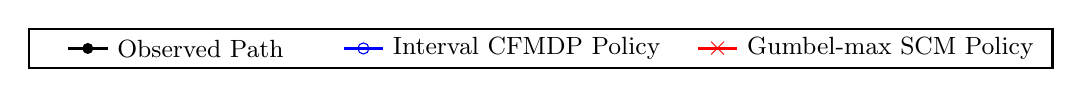
\begin{tikzpicture}[scale=1.0, every node/.style={scale=1.0}]
            \draw[thick, black] (-3, -0.25) rectangle (10, 0.25);
            %
            \draw[black, line width=1pt] (-2.5, 0.0) -- (-2,0.0);
            \fill[black] (-2.25,0.0) circle (2pt); %
            \node[right] at (-2,0.0) {\small Observed Path};
            
            %
            \draw[blue, line width=1pt] (1.0,0.0) -- (1.5,0.0);
            \node[draw=blue, circle, minimum size=4pt, inner sep=0pt] at (1.25,0.0) {}; %
            \node[right] at (1.5,0.0) {\small Interval CFMDP Policy};
            
            %
            \draw[red, line width=1pt] (5.5,0) -- (6,0);
            \node[red] at (5.75,0) {$\boldsymbol{\times}$}; %
            \node[right] at (6,0) {\small Gumbel-max SCM Policy};
        \end{tikzpicture}
    }\\
    %
    \subfigure[\footnotesize Lowest cumulative reward: Interval CFMDP ($312$), Gumbel-max SCM ($312$)]{%
        \resizebox{0.76\columnwidth}{!}{
             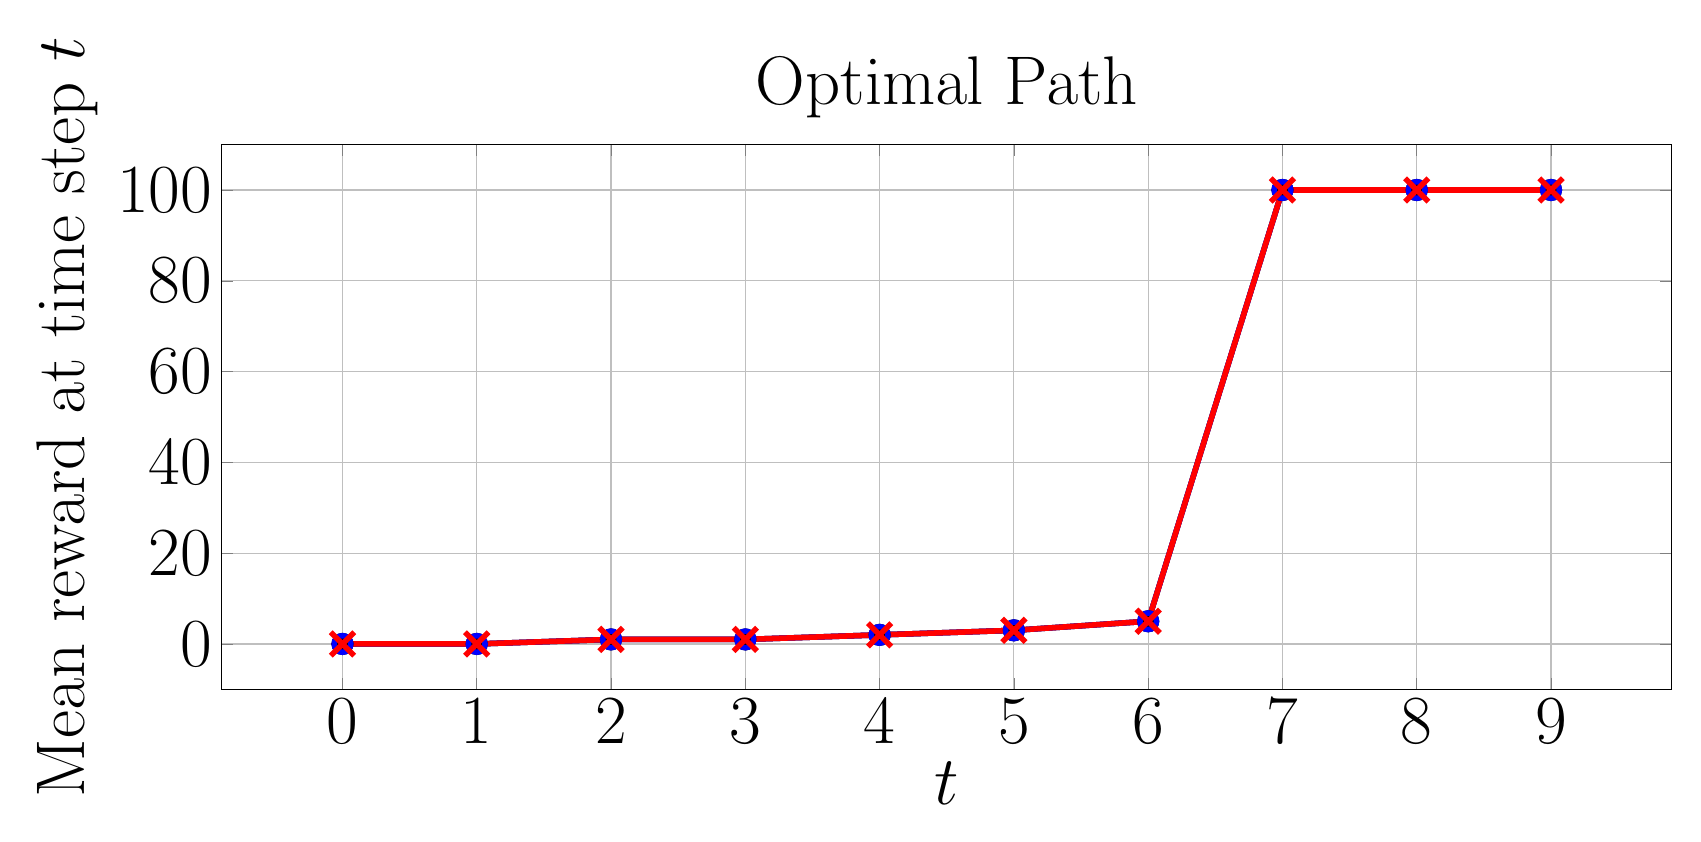
\begin{tikzpicture}
                \begin{axis}[
                    xlabel={$t$},
                    ylabel={Mean reward at time step $t$},
                    title={Optimal Path},
                    grid=both,
                    width=20cm, height=8.5cm,
                    every axis/.style={font=\Huge},
                    %
                ]
                \addplot[
                    color=black, %
                    mark=*, %
                    line width=2pt,
                    mark size=3pt,
                    error bars/.cd,
                    y dir=both, %
                    y explicit, %
                    error bar style={line width=1pt,solid},
                    error mark options={line width=1pt,mark size=4pt,rotate=90}
                ]
                coordinates {
                    (0, 0.0)  +- (0, 0.0)
                    (1, 0.0)  +- (0, 0.0) 
                    (2, 1.0)  +- (0, 0.0) 
                    (3, 1.0)  +- (0, 0.0)
                    (4, 2.0)  +- (0, 0.0)
                    (5, 3.0) +- (0, 0.0)
                    (6, 5.0) +- (0, 0.0)
                    (7, 100.0) +- (0, 0.0)
                    (8, 100.0) +- (0, 0.0)
                    (9, 100.0) +- (0, 0.0)
                };
                %
                \addplot[
                    color=blue, %
                    mark=o, %
                    line width=2pt,
                    mark size=3pt,
                    error bars/.cd,
                    y dir=both, %
                    y explicit, %
                    error bar style={line width=1pt,solid},
                    error mark options={line width=1pt,mark size=4pt,rotate=90}
                ]
                 coordinates {
                    (0, 0.0)  +- (0, 0.0)
                    (1, 0.0)  +- (0, 0.0) 
                    (2, 1.0)  +- (0, 0.0) 
                    (3, 1.0)  +- (0, 0.0)
                    (4, 2.0)  +- (0, 0.0)
                    (5, 3.0) +- (0, 0.0)
                    (6, 5.0) +- (0, 0.0)
                    (7, 100.0) +- (0, 0.0)
                    (8, 100.0) +- (0, 0.0)
                    (9, 100.0) +- (0, 0.0)
                };
                %
                \addplot[
                    color=red, %
                    mark=x, %
                    line width=2pt,
                    mark size=6pt,
                    error bars/.cd,
                    y dir=both, %
                    y explicit, %
                    error bar style={line width=1pt,solid},
                    error mark options={line width=1pt,mark size=4pt,rotate=90}
                ]
                coordinates {
                    (0, 0.0)  +- (0, 0.0)
                    (1, 0.0)  +- (0, 0.0) 
                    (2, 1.0)  +- (0, 0.0) 
                    (3, 1.0)  +- (0, 0.0)
                    (4, 2.0)  +- (0, 0.0)
                    (5, 3.0) +- (0, 0.0)
                    (6, 5.0) +- (0, 0.0)
                    (7, 100.0) +- (0, 0.0)
                    (8, 100.0) +- (0, 0.0)
                    (9, 100.0) +- (0, 0.0)
                };
                \end{axis}
            \end{tikzpicture}
         }
    }
    \hspace{1cm}
    \subfigure[\footnotesize Lowest cumulative reward: Interval CFMDP ($19$), Gumbel-max SCM ($-88$)]{%
         \resizebox{0.76\columnwidth}{!}{
            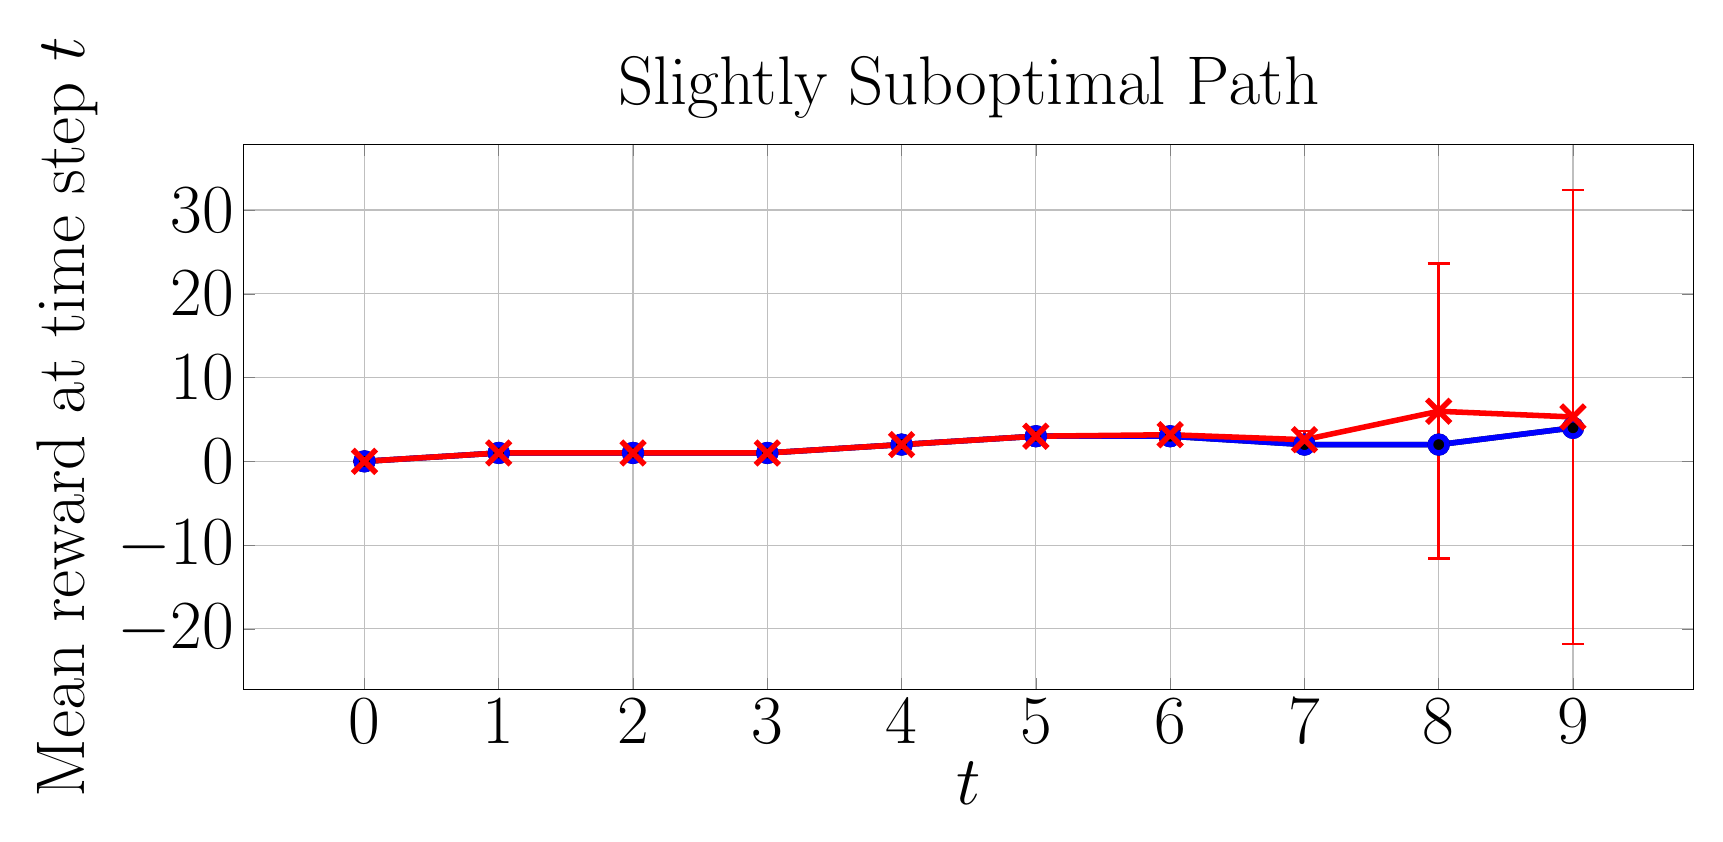
\begin{tikzpicture}
                \begin{axis}[
                    xlabel={$t$},
                    ylabel={Mean reward at time step $t$},
                    title={Slightly Suboptimal Path},
                    grid=both,
                    width=20cm, height=8.5cm,
                    every axis/.style={font=\Huge},
                    %
                ]
                \addplot[
                    color=black, %
                    mark=*, %
                    line width=2pt,
                    mark size=3pt,
                    error bars/.cd,
                    y dir=both, %
                    y explicit, %
                    error bar style={line width=1pt,solid},
                    error mark options={line width=1pt,mark size=4pt,rotate=90}
                ]
              coordinates {
                    (0, 0.0)  +- (0, 0.0)
                    (1, 1.0)  +- (0, 0.0) 
                    (2, 1.0)  +- (0, 0.0) 
                    (3, 1.0)  +- (0, 0.0)
                    (4, 2.0)  +- (0, 0.0)
                    (5, 3.0) +- (0, 0.0)
                    (6, 3.0) +- (0, 0.0)
                    (7, 2.0) +- (0, 0.0)
                    (8, 2.0) +- (0, 0.0)
                    (9, 4.0) +- (0, 0.0)
                };
                %
                \addplot[
                    color=blue, %
                    mark=o, %
                    line width=2pt,
                    mark size=3pt,
                    error bars/.cd,
                    y dir=both, %
                    y explicit, %
                    error bar style={line width=1pt,solid},
                    error mark options={line width=1pt,mark size=4pt,rotate=90}
                ]
              coordinates {
                    (0, 0.0)  +- (0, 0.0)
                    (1, 1.0)  +- (0, 0.0) 
                    (2, 1.0)  +- (0, 0.0) 
                    (3, 1.0)  +- (0, 0.0)
                    (4, 2.0)  +- (0, 0.0)
                    (5, 3.0) +- (0, 0.0)
                    (6, 3.0) +- (0, 0.0)
                    (7, 2.0) +- (0, 0.0)
                    (8, 2.0) +- (0, 0.0)
                    (9, 4.0) +- (0, 0.0)
                };
                %
                \addplot[
                    color=red, %
                    mark=x, %
                    line width=2pt,
                    mark size=6pt,
                    error bars/.cd,
                    y dir=both, %
                    y explicit, %
                    error bar style={line width=1pt,solid},
                    error mark options={line width=1pt,mark size=4pt,rotate=90}
                ]
                coordinates {
                    (0, 0.0)  +- (0, 0.0)
                    (1, 1.0)  +- (0, 0.0) 
                    (2, 1.0)  +- (0, 0.0) 
                    (3, 1.0)  +- (0, 0.0)
                    (4, 2.0)  += (0, 0.0)
                    (5, 3.0)  += (0, 0.0)
                    (6, 3.17847) += (0, 0.62606746) -= (0, 0.62606746)
                    (7, 2.5832885) += (0, 1.04598233) -= (0, 1.04598233)
                    (8, 5.978909) += (0, 17.60137623) -= (0, 17.60137623)
                    (9, 5.297059) += (0, 27.09227512) -= (0, 27.09227512)
                };
                \end{axis}
            \end{tikzpicture}
         }
    }\\[-1.5pt]
    \subfigure[\footnotesize Lowest cumulative reward: Interval CFMDP ($14$), Gumbel-max SCM ($-598$)]{%
         \resizebox{0.76\columnwidth}{!}{
             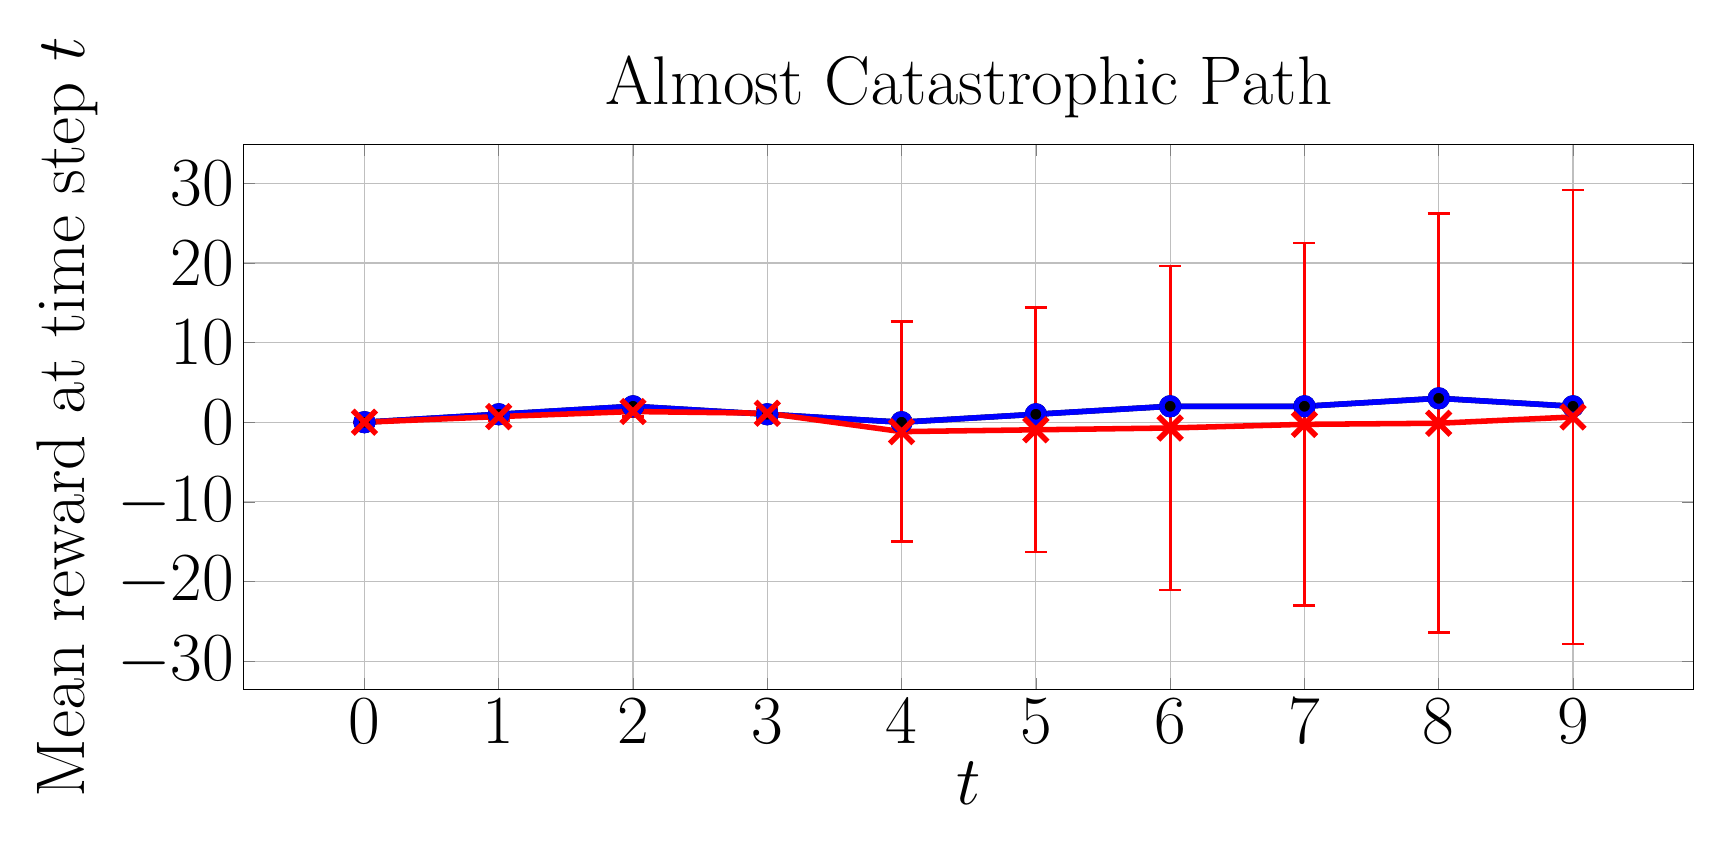
\begin{tikzpicture}
                \begin{axis}[
                    xlabel={$t$},
                    ylabel={Mean reward at time step $t$},
                    title={Almost Catastrophic Path},
                    grid=both,
                    width=20cm, height=8.5cm,
                    every axis/.style={font=\Huge},
                    %
                ]
                \addplot[
                    color=black, %
                    mark=*, %
                    line width=2pt,
                    mark size=3pt,
                    error bars/.cd,
                    y dir=both, %
                    y explicit, %
                    error bar style={line width=1pt,solid},
                    error mark options={line width=1pt,mark size=4pt,rotate=90}
                ]
                coordinates {
                    (0, 0.0)  +- (0, 0.0)
                    (1, 1.0)  +- (0, 0.0) 
                    (2, 2.0)  +- (0, 0.0) 
                    (3, 1.0)  +- (0, 0.0)
                    (4, 0.0)  +- (0, 0.0)
                    (5, 1.0) +- (0, 0.0)
                    (6, 2.0) +- (0, 0.0)
                    (7, 2.0) +- (0, 0.0)
                    (8, 3.0) +- (0, 0.0)
                    (9, 2.0) +- (0, 0.0)
                };
                %
                \addplot[
                    color=blue, %
                    mark=o, %
                    line width=2pt,
                    mark size=3pt,
                    error bars/.cd,
                    y dir=both, %
                    y explicit, %
                    error bar style={line width=1pt,solid},
                    error mark options={line width=1pt,mark size=4pt,rotate=90}
                ]
                coordinates {
                    (0, 0.0)  +- (0, 0.0)
                    (1, 1.0)  +- (0, 0.0) 
                    (2, 2.0)  +- (0, 0.0) 
                    (3, 1.0)  +- (0, 0.0)
                    (4, 0.0)  +- (0, 0.0)
                    (5, 1.0) +- (0, 0.0)
                    (6, 2.0) +- (0, 0.0)
                    (7, 2.0) +- (0, 0.0)
                    (8, 3.0) +- (0, 0.0)
                    (9, 2.0) +- (0, 0.0)
                };
                %
                \addplot[
                    color=red, %
                    mark=x, %
                    line width=2pt,
                    mark size=6pt,
                    error bars/.cd,
                    y dir=both, %
                    y explicit, %
                    error bar style={line width=1pt,solid},
                    error mark options={line width=1pt,mark size=4pt,rotate=90}
                ]
                coordinates {
                    (0, 0.0)  +- (0, 0.0)
                    (1, 0.7065655)  +- (0, 0.4553358) 
                    (2, 1.341673)  +- (0, 0.67091621) 
                    (3, 1.122926)  +- (0, 0.61281824)
                    (4, -1.1821935)  +- (0, 13.82444042)
                    (5, -0.952399)  +- (0, 15.35195457)
                    (6, -0.72672) +- (0, 20.33508414)
                    (7, -0.268983) +- (0, 22.77861454)
                    (8, -0.1310835) +- (0, 26.31013314)
                    (9, 0.65806) +- (0, 28.50670214)
                };
                %
            %
            %
            %
            %
            %
            %
            %
            %
            %
            %
            %
            %
            %
            %
            %
            %
            %
            %
                \end{axis}
            \end{tikzpicture}
         }
    }
    \hspace{1cm}
    \subfigure[\footnotesize Lowest cumulative reward: Interval CFMDP ($-698$), Gumbel-max SCM ($-698$)]{%
         \resizebox{0.76\columnwidth}{!}{
            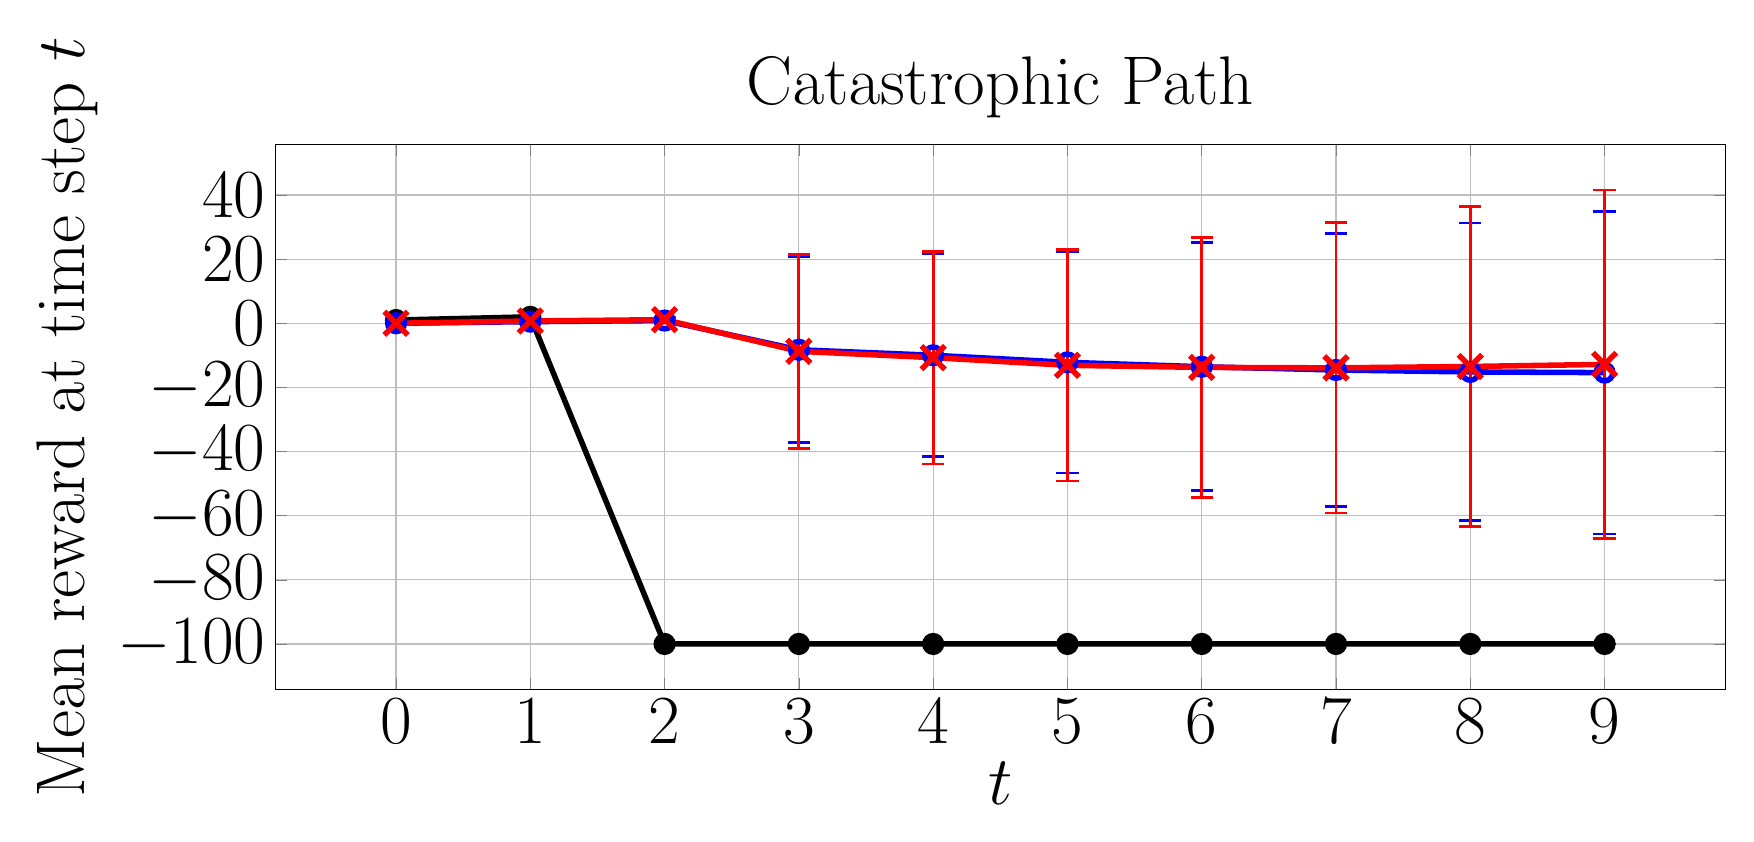
\begin{tikzpicture}
                \begin{axis}[
                    xlabel={$t$},
                    ylabel={Mean reward at time step $t$},
                    title={Catastrophic Path},
                    grid=both,
                    width=20cm, height=8.5cm,
                    every axis/.style={font=\Huge},
                    %
                ]
                \addplot[
                    color=black, %
                    mark=*, %
                    line width=2pt,
                    mark size=3pt,
                    error bars/.cd,
                    y dir=both, %
                    y explicit, %
                    error bar style={line width=1pt,solid},
                    error mark options={line width=1pt,mark size=4pt,rotate=90}
                ]
                coordinates {
                    (0, 1.0)  +- (0, 0.0)
                    (1, 2.0)  +- (0, 0.0) 
                    (2, -100.0)  +- (0, 0.0) 
                    (3, -100.0)  +- (0, 0.0)
                    (4, -100.0)  +- (0, 0.0)
                    (5, -100.0) +- (0, 0.0)
                    (6, -100.0) +- (0, 0.0)
                    (7, -100.0) +- (0, 0.0)
                    (8, -100.0) +- (0, 0.0)
                    (9, -100.0) +- (0, 0.0)
                };
                %
                \addplot[
                    color=blue, %
                    mark=o, %
                    line width=2pt,
                    mark size=3pt,
                    error bars/.cd,
                    y dir=both, %
                    y explicit, %
                    error bar style={line width=1pt,solid},
                    error mark options={line width=1pt,mark size=4pt,rotate=90}
                ]
                coordinates {
                    (0, 0.0)  +- (0, 0.0)
                    (1, 0.504814)  +- (0, 0.49997682) 
                    (2, 0.8439835)  +- (0, 0.76831917) 
                    (3, -8.2709165)  +- (0, 28.93656754)
                    (4, -9.981082)  +- (0, 31.66825363)
                    (5, -12.1776325) +- (0, 34.53463233)
                    (6, -13.556076) +- (0, 38.62845372)
                    (7, -14.574418) +- (0, 42.49603359)
                    (8, -15.1757075) +- (0, 46.41913968)
                    (9, -15.3900395) +- (0, 50.33563368)
                };
                %
                \addplot[
                    color=red, %
                    mark=x, %
                    line width=2pt,
                    mark size=6pt,
                    error bars/.cd,
                    y dir=both, %
                    y explicit, %
                    error bar style={line width=1pt,solid},
                    error mark options={line width=1pt,mark size=4pt,rotate=90}
                ]
                coordinates {
                    (0, 0.0)  +- (0, 0.0)
                    (1, 0.701873)  +- (0, 0.45743556) 
                    (2, 1.1227805)  +- (0, 0.73433129) 
                    (3, -8.7503255)  +- (0, 30.30257976)
                    (4, -10.722092)  +- (0, 33.17618589)
                    (5, -13.10721)  +- (0, 36.0648089)
                    (6, -13.7631645) +- (0, 40.56553451)
                    (7, -13.909043) +- (0, 45.23829402)
                    (8, -13.472517) +- (0, 49.96270296)
                    (9, -12.8278835) +- (0, 54.38618735)
                };
                %
            %
            %
            %
            %
            %
            %
            %
            %
            %
            %
            %
            %
            %
            %
            %
            %
            %
            %
                \end{axis}
            \end{tikzpicture}
         }
    }
    \caption{Average instant reward of CF paths induced by policies on GridWorld $p=0.4$.}
    \label{fig: reward p=0.4}
\end{figure*}

\subsection{Experimental Setup}
To compare policy performance, we measure the average rewards of counterfactual paths induced by our policy and the Gumbel-max policy by uniformly sampling $200$ counterfactual MDPs from the ICFMDP and generating $10,000$ counterfactual paths over each sampled CFMDP. \jl{Since the interval CFMDP depends on the observed path, we select $4$  paths of varying optimality to evaluate how the observed path impacts the performance of both policies: an optimal path, a slightly suboptimal path that could reach the optimal reward with a few changes, a catastrophic path that enters a catastrophic, terminal state with low reward, and an almost catastrophic path that was close to entering a catastrophic state.} When measuring the average probability bound widths and execution time needed to generate the ICFMDPs, we averaged over $20$ randomly generated observed paths
\footnote{Further training details are provided in Appendix \ref{app: training details}, and the code is provided at \href{https://github.com/ddv-lab/robust-cf-inference-in-MDPs}{https://github.com/ddv-lab/robust-cf-inference-in-MDPs}
%
%
.}.

\subsection{GridWorld}
\jl{The GridWorld MDP is a $4 \times 4$ grid where an agent must navigate from the top-left corner to the goal state in the bottom-right corner, avoiding a dangerous terminal state in the centre. At each time step, the agent can move up, down, left, or right, but there is a small probability (controlled by hyper-parameter $p$) of moving in an unintended direction. As the agent nears the goal, the reward for each state increases, culminating in a reward of $+100$ for reaching the goal. Entering the dangerous state results in a penalty of $-100$. We use two versions of GridWorld: a less stochastic version with $p=0.9$ (i.e., $90$\% chance of moving in the chosen direction) and a more stochastic version with $p=0.4$.}

\paragraph{GridWorld ($p=0.9$)}
When $p=0.9$, the counterfactual probability bounds are typically narrow (see Table \ref{tab:nonzero_probs} for average measurements). Consequently, as shown in Figure \ref{fig: reward p=0.9}, both policies are nearly identical and perform similarly well across the optimal, slightly suboptimal, and catastrophic paths.
%
However, for the almost catastrophic path, the interval CFMDP path is more conservative and follows the observed path more closely (as this is where the probability bounds are narrowest), which typically requires one additional step to reach the goal state than the Gumbel-max SCM policy.
%

\paragraph{GridWorld ($p=0.4$)}
\jl{When $p=0.4$, the GridWorld environment becomes more uncertain, increasing the risk of entering the dangerous state even if correct actions are chosen. Thus, as shown in Figure \ref{fig: reward p=0.4}, the interval CFMDP policy adopts a more conservative approach, avoiding deviation from the observed policy if it cannot guarantee higher counterfactual rewards (see the slightly suboptimal and almost catastrophic paths), whereas the Gumbel-max SCM is inconsistent: it can yield higher rewards, but also much lower rewards, reflected in the wide error bars.} For the catastrophic path, both policies must deviate from the observed path to achieve a higher reward and, in this case, perform similarly.
%
%
%
%
\subsection{Sepsis}
The Sepsis MDP \citep{oberst2019counterfactual} simulates trajectories of Sepsis patients. Each state consists of four vital signs (heart rate, blood pressure, oxygen concentration, and glucose levels), categorised as low, normal, or high.
and three treatments that can be toggled on/off at each time step (8 actions in total). Unlike \citet{oberst2019counterfactual}, we scale rewards based on the number of out-of-range vital signs, between $-1000$ (patient dies) and $1000$ (patient discharged). \jl{Like the GridWorld $p=0.4$ experiment, the Sepsis MDP is highly uncertain, as many states are equally likely to lead to optimal and poor outcomes. Thus, as shown in Figure \ref{fig: reward sepsis}, both policies follow the observed optimal and almost catastrophic paths to guarantee rewards are no worse than the observation.} However, improving the catastrophic path requires deviating from the observation. Here, the Gumbel-max SCM policy, on average, performs better than the interval CFMDP policy. But, since both policies have lower bounds clipped at $-1000$, neither policy reliably improves over the observation. In contrast, for the slightly suboptimal path, the interval CFMDP policy performs significantly better, shown by its higher lower bounds. 
Moreover, in these two cases, the worst-case counterfactual path generated by the interval CFMDP policy is better than that of the Gumbel-max SCM policy,
indicating its greater robustness.
%
\begin{figure*}
    \centering
     \resizebox{0.6\textwidth}{!}{
        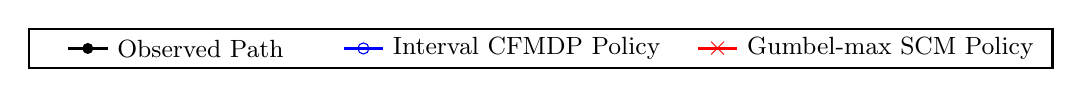
\begin{tikzpicture}[scale=1.0, every node/.style={scale=1.0}]
            \draw[thick, black] (-3, -0.25) rectangle (10, 0.25);
            %
            \draw[black, line width=1pt] (-2.5, 0.0) -- (-2,0.0);
            \fill[black] (-2.25,0.0) circle (2pt); %
            \node[right] at (-2,0.0) {\small Observed Path};
            
            %
            \draw[blue, line width=1pt] (1.0,0.0) -- (1.5,0.0);
            \node[draw=blue, circle, minimum size=4pt, inner sep=0pt] at (1.25,0.0) {}; %
            \node[right] at (1.5,0.0) {\small Interval CFMDP Policy};
            
            %
            \draw[red, line width=1pt] (5.5,0) -- (6,0);
            \node[red] at (5.75,0) {$\boldsymbol{\times}$}; %
            \node[right] at (6,0) {\small Gumbel-max SCM Policy};
        \end{tikzpicture}
    }\\
    \subfigure[\footnotesize Lowest cumulative reward: Interval CFMDP ($8000$), Gumbel-max SCM ($8000$)]{%
         \resizebox{0.76\columnwidth}{!}{
             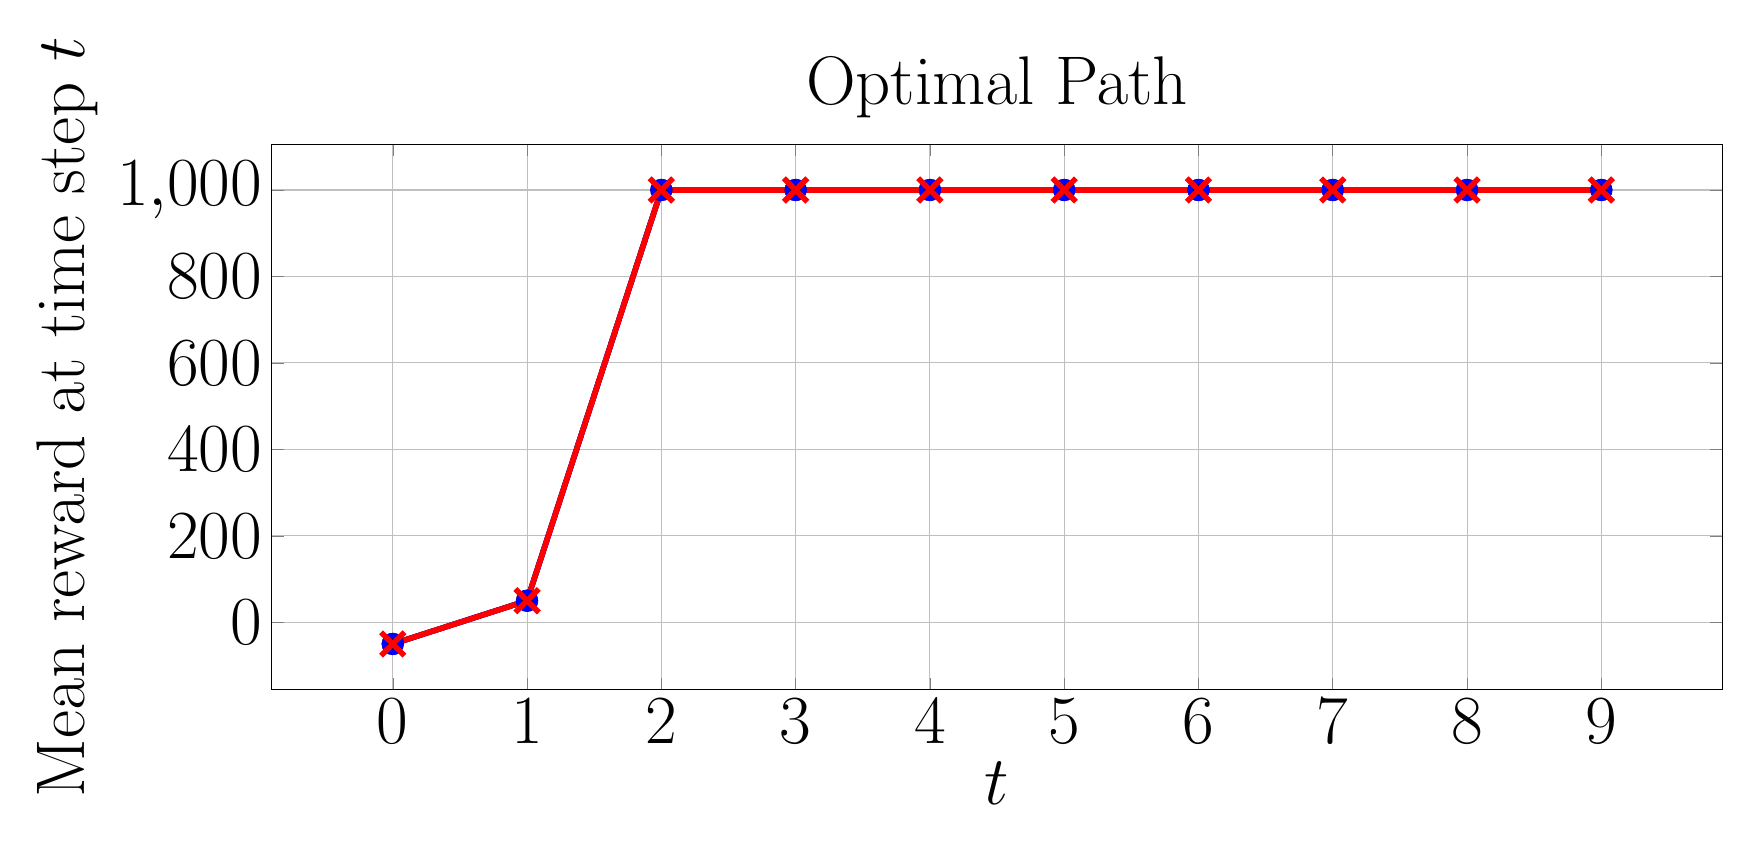
\begin{tikzpicture}
                \begin{axis}[
                    xlabel={$t$},
                    ylabel={Mean reward at time step $t$},
                    title={Optimal Path},
                    grid=both,
                    width=20cm, height=8.5cm,
                    every axis/.style={font=\Huge},
                    %
                ]
                \addplot[
                    color=black, %
                    mark=*, %
                    line width=2pt,
                    mark size=3pt,
                ]
                coordinates {
                    (0, -50.0)
                    (1, 50.0)
                    (2, 1000.0)
                    (3, 1000.0)
                    (4, 1000.0)
                    (5, 1000.0)
                    (6, 1000.0)
                    (7, 1000.0)
                    (8, 1000.0)
                    (9, 1000.0)
                };
                %
                \addplot[
                    color=blue, %
                    mark=o, %
                    line width=2pt,
                    mark size=3pt,
                    error bars/.cd,
                    y dir=both, %
                    y explicit, %
                    error bar style={line width=1pt,solid},
                    error mark options={line width=1pt,mark size=4pt,rotate=90}
                ]
                coordinates {
                    (0, -50.0)  +- (0, 0.0)
                    (1, 50.0)  +- (0, 0.0) 
                    (2, 1000.0)  +- (0, 0.0) 
                    (3, 1000.0)  +- (0, 0.0)
                    (4, 1000.0)  +- (0, 0.0)
                    (5, 1000.0) +- (0, 0.0)
                    (6, 1000.0) +- (0, 0.0)
                    (7, 1000.0) +- (0, 0.0)
                    (8, 1000.0) +- (0, 0.0)
                    (9, 1000.0) +- (0, 0.0)
                };
                %
                \addplot[
                    color=red, %
                    mark=x, %
                    line width=2pt,
                    mark size=6pt,
                    error bars/.cd,
                    y dir=both, %
                    y explicit, %
                    error bar style={line width=1pt,solid},
                    error mark options={line width=1pt,mark size=4pt,rotate=90}
                ]
                coordinates {
                    (0, -50.0)  +- (0, 0.0)
                    (1, 50.0)  +- (0, 0.0) 
                    (2, 1000.0)  +- (0, 0.0) 
                    (3, 1000.0)  +- (0, 0.0)
                    (4, 1000.0)  +- (0, 0.0)
                    (5, 1000.0) +- (0, 0.0)
                    (6, 1000.0) +- (0, 0.0)
                    (7, 1000.0) +- (0, 0.0)
                    (8, 1000.0) +- (0, 0.0)
                    (9, 1000.0) +- (0, 0.0)
                };
                %
                \end{axis}
            \end{tikzpicture}
         }
    }
    \hspace{1cm}
    \subfigure[\footnotesize Lowest cumulative reward: Interval CFMDP ($-5980$), Gumbel-max SCM ($-8000$)]{%
         \resizebox{0.76\columnwidth}{!}{
            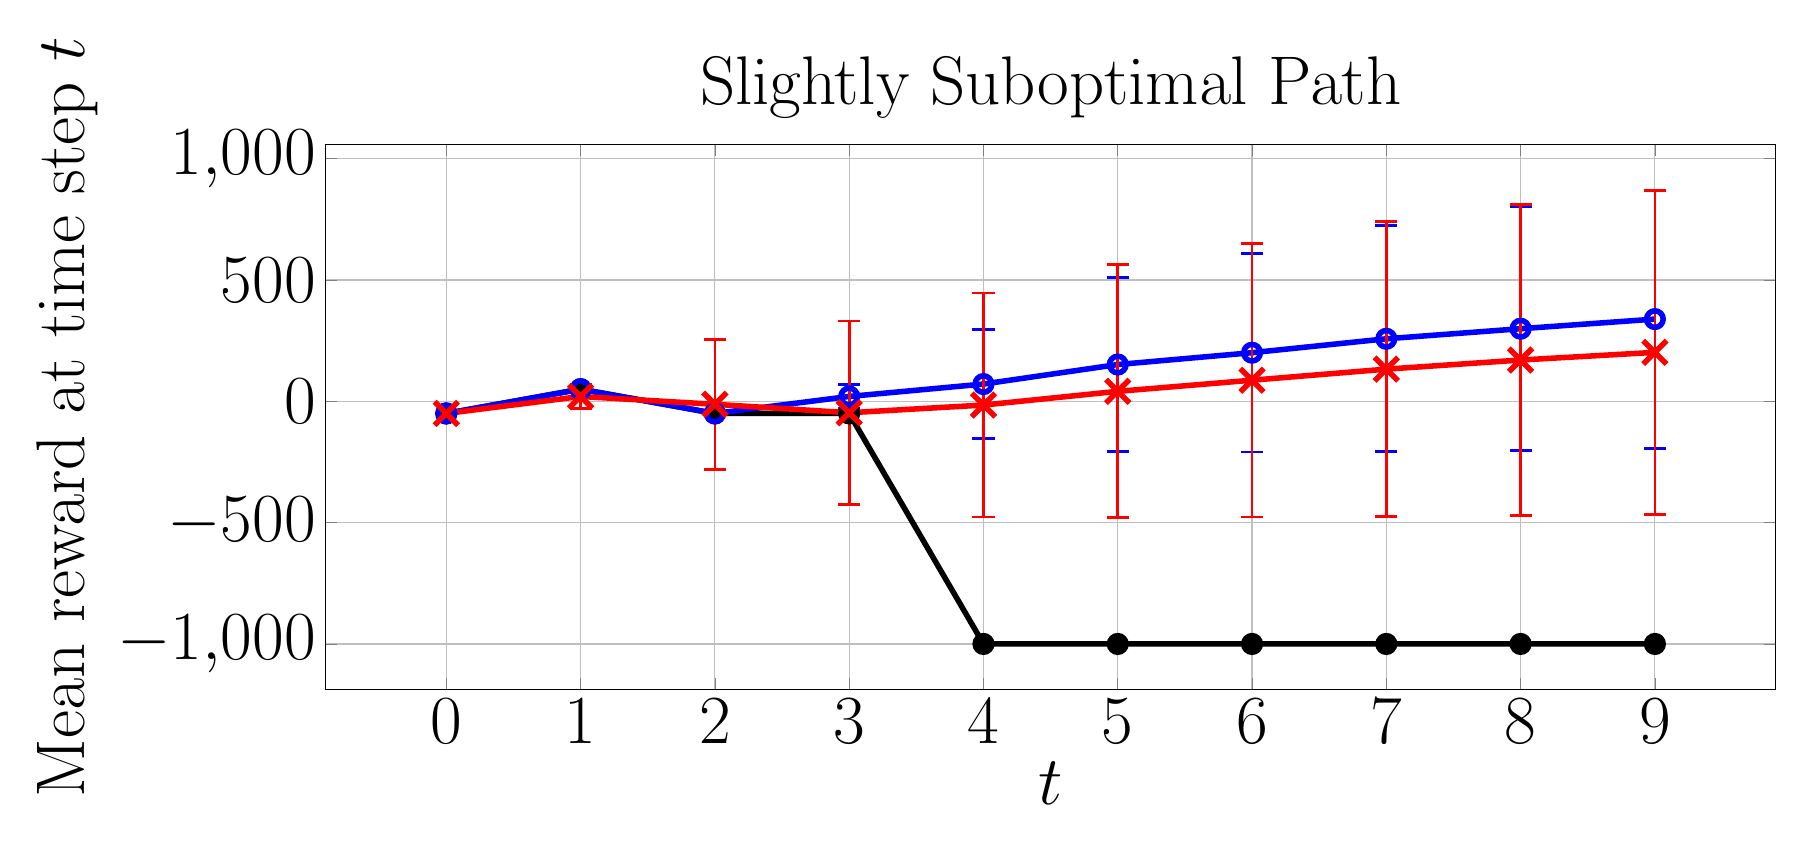
\begin{tikzpicture}
                \begin{axis}[
                    xlabel={$t$},
                    ylabel={Mean reward at time step $t$},
                    title={Slightly Suboptimal Path},
                    grid=both,
                    width=20cm, height=8.5cm,
                    every axis/.style={font=\Huge},
                    %
                ]
               \addplot[
                    color=black, %
                    mark=*, %
                    line width=2pt,
                    mark size=3pt,
                ]
                coordinates {
                    (0, -50.0)
                    (1, 50.0)
                    (2, -50.0)
                    (3, -50.0)
                    (4, -1000.0)
                    (5, -1000.0)
                    (6, -1000.0)
                    (7, -1000.0)
                    (8, -1000.0)
                    (9, -1000.0)
                };
                %
                \addplot[
                    color=blue, %
                    mark=o, %
                    line width=2pt,
                    mark size=3pt,
                    error bars/.cd,
                    y dir=both, %
                    y explicit, %
                    error bar style={line width=1pt,solid},
                    error mark options={line width=1pt,mark size=4pt,rotate=90}
                ]
                coordinates {
                    (0, -50.0)  +- (0, 0.0)
                    (1, 50.0)  +- (0, 0.0) 
                    (2, -50.0)  +- (0, 0.0) 
                    (3, 20.0631)  +- (0, 49.97539413)
                    (4, 71.206585)  +- (0, 226.02033693)
                    (5, 151.60797) +- (0, 359.23292559)
                    (6, 200.40593) +- (0, 408.86185176)
                    (7, 257.77948) +- (0, 466.10372804)
                    (8, 299.237465) +- (0, 501.82579506)
                    (9, 338.9129) +- (0, 532.06124996)
                };
                %
                \addplot[
                    color=red, %
                    mark=x, %
                    line width=2pt,
                    mark size=6pt,
                    error bars/.cd,
                    y dir=both, %
                    y explicit, %
                    error bar style={line width=1pt,solid},
                    error mark options={line width=1pt,mark size=4pt,rotate=90}
                ]
                coordinates {
                    (0, -50.0)  +- (0, 0.0)
                    (1, 20.00736)  +- (0, 49.99786741) 
                    (2, -12.282865)  +- (0, 267.598755) 
                    (3, -47.125995)  +- (0, 378.41755832)
                    (4, -15.381965)  +- (0, 461.77616558)
                    (5, 41.15459) +- (0, 521.53189262)
                    (6, 87.01595) +- (0, 564.22243126 )
                    (7, 132.62376) +- (0, 607.31338037)
                    (8, 170.168145) +- (0, 641.48013693)
                    (9, 201.813135) +- (0, 667.29441777)
                };
                %
                %
                %
                %
                %
                %
                %
                %
                %
                %
                %
                %
                %
                %
                %
                %
                %
                %
                %
                \end{axis}
            \end{tikzpicture}
         }
    }\\[-1.5pt]
    \subfigure[\footnotesize Lowest cumulative reward: Interval CFMDP ($100$), Gumbel-max SCM ($100$)]{%
         \resizebox{0.76\columnwidth}{!}{
             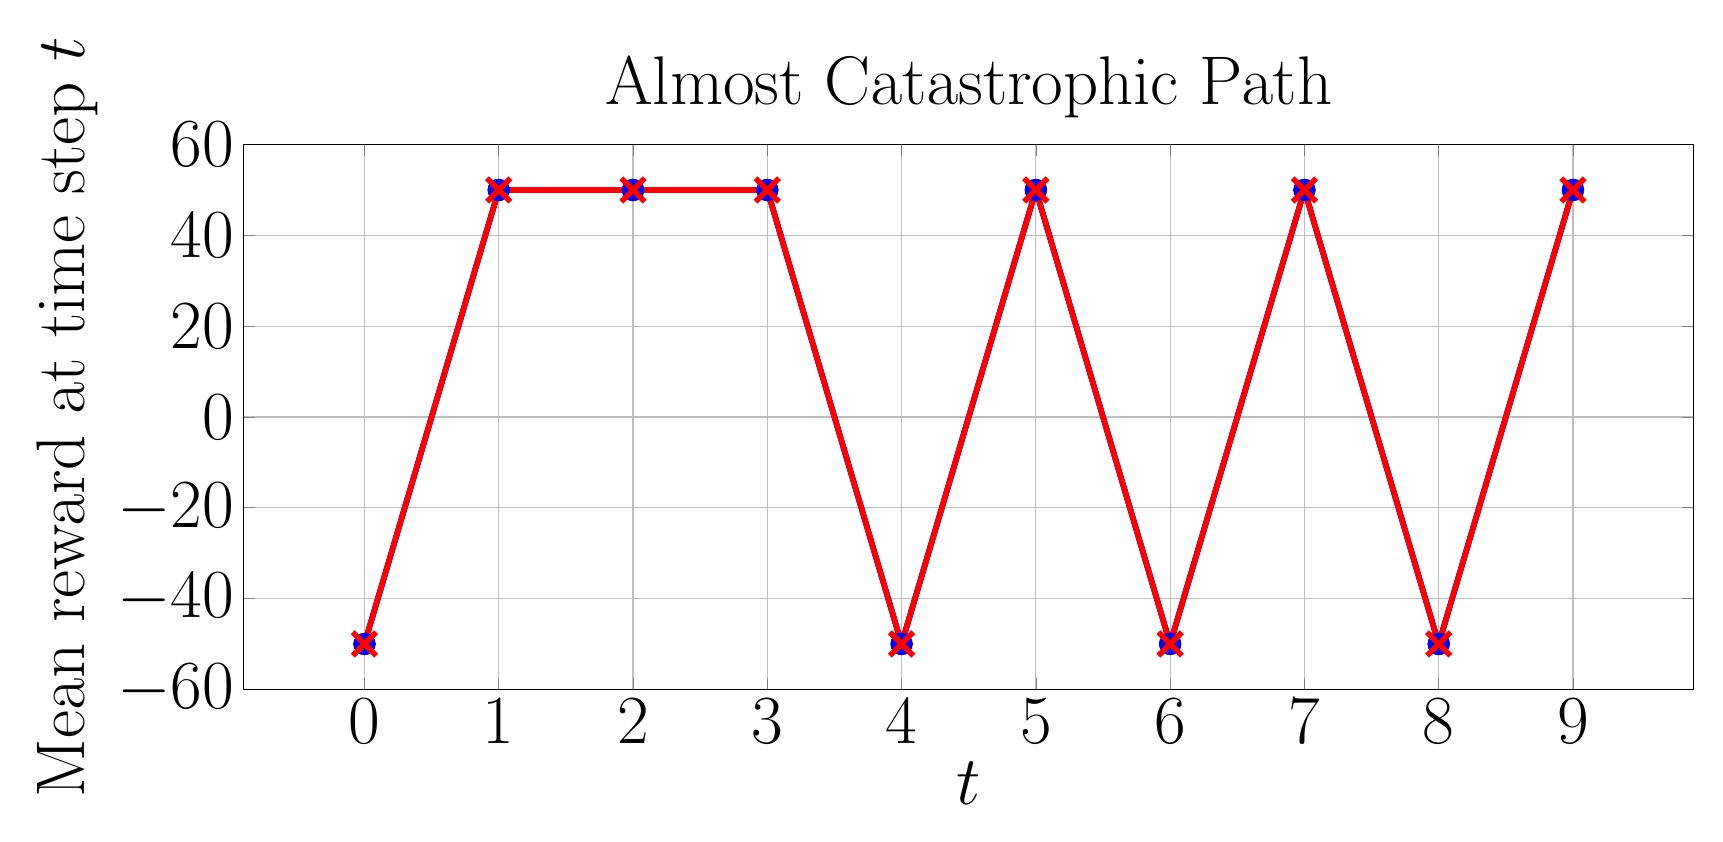
\begin{tikzpicture}
                \begin{axis}[
                    xlabel={$t$},
                    ylabel={Mean reward at time step $t$},
                    title={Almost Catastrophic Path},
                    grid=both,
                    every axis/.style={font=\Huge},
                    width=20cm, height=8.5cm,
                    %
                ]
               \addplot[
                    color=black, %
                    mark=*, %
                    line width=2pt,
                    mark size=3pt,
                ]
                coordinates {
                    (0, -50.0)
                    (1, 50.0)
                    (2, 50.0)
                    (3, 50.0)
                    (4, -50.0)
                    (5, 50.0)
                    (6, -50.0)
                    (7, 50.0)
                    (8, -50.0)
                    (9, 50.0)
                };
                %
                %
                \addplot[
                    color=blue, %
                    mark=o, %
                    line width=2pt,
                    mark size=3pt,
                    error bars/.cd,
                    y dir=both, %
                    y explicit, %
                    error bar style={line width=1pt,solid},
                    error mark options={line width=1pt,mark size=4pt,rotate=90}
                ]
                coordinates {
                    (0, -50.0)  +- (0, 0.0)
                    (1, 50.0)  +- (0, 0.0) 
                    (2, 50.0)  +- (0, 0.0) 
                    (3, 50.0)  +- (0, 0.0)
                    (4, -50.0)  +- (0, 0.0)
                    (5, 50.0) +- (0, 0.0)
                    (6, -50.0) +- (0, 0.0)
                    (7, 50.0) +- (0, 0.0)
                    (8, -50.0) +- (0, 0.0)
                    (9, 50.0) +- (0, 0.0)
                };
                %
                \addplot[
                    color=red, %
                    mark=x, %
                    line width=2pt,
                    mark size=6pt,
                    error bars/.cd,
                    y dir=both, %
                    y explicit, %
                    error bar style={line width=1pt,solid},
                    error mark options={line width=1pt,mark size=4pt,rotate=90}
                ]
                coordinates {
                    (0, -50.0)  +- (0, 0.0)
                    (1, 50.0)  +- (0, 0.0) 
                    (2, 50.0)  +- (0, 0.0) 
                    (3, 50.0)  +- (0, 0.0)
                    (4, -50.0)  +- (0, 0.0)
                    (5, 50.0) +- (0, 0.0)
                    (6, -50.0) +- (0, 0.0)
                    (7, 50.0) +- (0, 0.0)
                    (8, -50.0) +- (0, 0.0)
                    (9, 50.0) +- (0, 0.0)
                };
                %
                %
                %
                %
                %
                %
                %
                %
                %
                %
                %
                %
                %
                %
                %
                %
                %
                %
                %
                \end{axis}
            \end{tikzpicture}
         }
    }
    \hspace{1cm}
    \subfigure[\footnotesize Lowest cumulative reward: Interval CFMDP ($-7150$), Gumbel-max SCM ($-9050$)]{%
         \resizebox{0.76\columnwidth}{!}{
            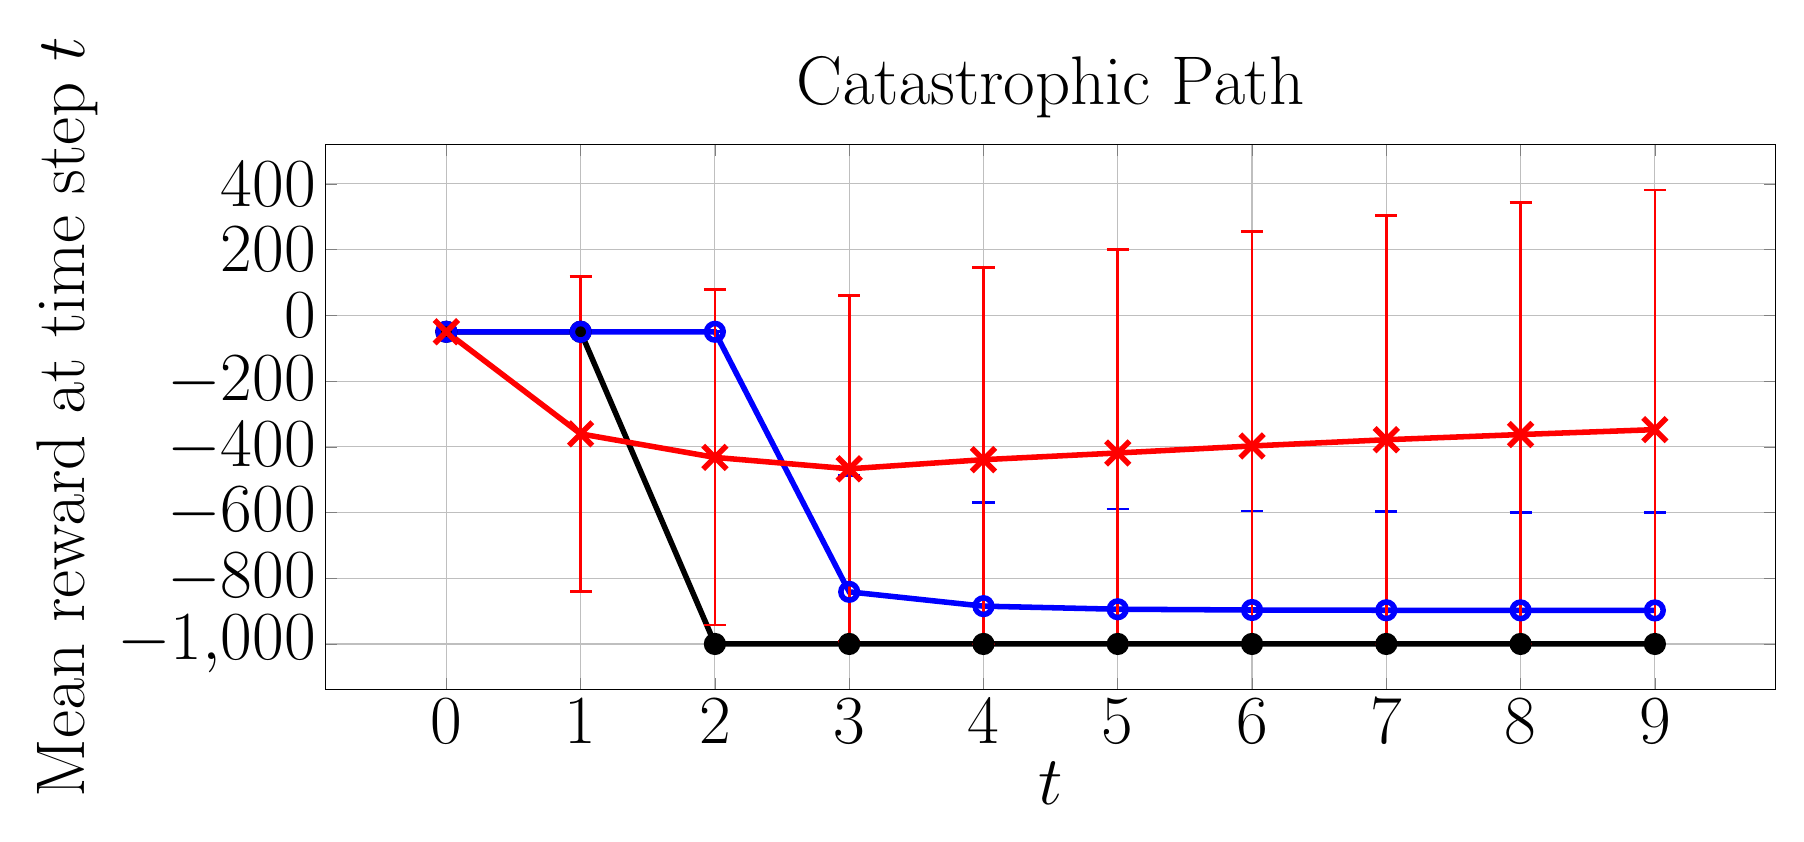
\begin{tikzpicture}
                \begin{axis}[
                    xlabel={$t$},
                    ylabel={Mean reward at time step $t$},
                    title={Catastrophic Path},
                    grid=both,
                    width=20cm, height=8.5cm,
                    every axis/.style={font=\Huge},
                    %
                ]
               \addplot[
                    color=black, %
                    mark=*, %
                    line width=2pt,
                    mark size=3pt,
                ]
                coordinates {
                    (0, -50.0)
                    (1, -50.0)
                    (2, -1000.0)
                    (3, -1000.0)
                    (4, -1000.0)
                    (5, -1000.0)
                    (6, -1000.0)
                    (7, -1000.0)
                    (8, -1000.0)
                    (9, -1000.0)
                };
                %
                %
                \addplot[
                    color=blue, %
                    mark=o, %
                    line width=2pt,
                    mark size=3pt,
                    error bars/.cd,
                    y dir=both, %
                    y explicit, %
                    error bar style={line width=1pt,solid},
                    error mark options={line width=1pt,mark size=4pt,rotate=90}
                ]
                coordinates {
                    (0, -50.0)  +- (0, 0.0)
                    (1, -50.0)  +- (0, 0.0) 
                    (2, -50.0)  +- (0, 0.0) 
                    (3, -841.440725)  += (0, 354.24605512) -= (0, 158.559275)
                    (4, -884.98225)  += (0, 315.37519669) -= (0, 115.01775)
                    (5, -894.330425) += (0, 304.88572805) -= (0, 105.669575)
                    (6, -896.696175) += (0, 301.19954514) -= (0, 103.303825)
                    (7, -897.4635) += (0, 299.61791279) -= (0, 102.5365)
                    (8, -897.77595) += (0, 298.80392585) -= (0, 102.22405)
                    (9, -897.942975) += (0, 298.32920557) -= (0, 102.057025)
                };
                %
                \addplot[
                    color=red, %
                    mark=x, %
                    line width=2pt,
                    mark size=6pt,
                    error bars/.cd,
                    y dir=both, %
                    y explicit, %
                    error bar style={line width=1pt,solid},
                    error mark options={line width=1pt,mark size=4pt,rotate=90}
                ]
            coordinates {
                    (0, -50.0)  +- (0, 0.0)
                    (1, -360.675265)  +- (0, 479.39812699) 
                    (2, -432.27629)  +- (0, 510.38620897) 
                    (3, -467.029545)  += (0, 526.36009628) -= (0, 526.36009628)
                    (4, -439.17429)  += (0, 583.96638919) -= (0, 560.82571)
                    (5, -418.82704) += (0, 618.43027478) -= (0, 581.17296)
                    (6, -397.464895) += (0, 652.67322574) -= (0, 602.535105)
                    (7, -378.49052) += (0, 682.85407033) -= (0, 621.50948)
                    (8, -362.654195) += (0, 707.01412023) -= (0, 637.345805)
                    (9, -347.737935) += (0, 729.29076479) -= (0, 652.262065)
                };
                %
                %
                %
                %
                %
                %
                %
                %
                %
                %
                %
                %
                %
                %
                %
                %
                %
                %
                %
                \end{axis}
            \end{tikzpicture}
         }
    }
    \caption{Average instant reward of CF paths induced by policies on Sepsis.}
    \label{fig: reward sepsis}
\end{figure*}

%
%
%
\subsection{Interval CFMDP Bounds}
%
%
Table \ref{tab:nonzero_probs} presents the mean counterfactual probability bound widths (excluding transitions where the upper bound is $0$) for each MDP, averaged over 20 observed paths. We compare the bounds under counterfactual stability (CS) and monotonicity (M) assumptions, CS alone, and no assumptions. This shows that the assumptions marginally reduce the bound widths, indicating the assumptions tighten the bounds without excluding too many causal models, as intended.
\renewcommand{\arraystretch}{1}

\begin{table}
\centering
\caption{Mean width of counterfactual probability bounds}
\resizebox{0.8\columnwidth}{!}{%
\begin{tabular}{|c|c|c|c|}
\hline
\multirow{2}{*}{\textbf{Environment}} & \multicolumn{3}{c|}{\textbf{Assumptions}} \\ \cline{2-4}
 & \textbf{CS + M} & \textbf{CS} & \textbf{None\tablefootnote{\jl{Equivalent to \citet{li2024probabilities}'s bounds (see Section \ref{sec: equivalence with Li}).}}} \\ \hline
\textbf{GridWorld} ($p=0.9$) & 0.0817 & 0.0977 & 0.100 \\ \hline
\textbf{GridWorld} ($p=0.4$) & 0.552  & 0.638  & 0.646 \\ \hline
\textbf{Sepsis} & 0.138 & 0.140 & 0.140 \\ \hline
\end{tabular}
}
\label{tab:nonzero_probs}
\end{table}


\subsection{Execution Times}
Table \ref{tab: times} compares the average time needed to generate the interval CFMDP vs.\ the Gumbel-max SCM CFMDP for 20 observations.
The GridWorld algorithms were run single-threaded, while the Sepsis experiments were run in parallel.
Generating the interval CFMDP is significantly faster as it uses exact analytical bounds, whereas the Gumbel-max CFMDP requires sampling from the Gumbel distribution to estimate counterfactual transition probabilities. \jl{Since constructing the counterfactual MDP models is the main bottleneck in both approaches, ours is more efficient overall and suitable for larger MDPs.}
\begin{table}
\centering
\caption{Mean execution time to generate CFMDPs}
\resizebox{0.99\columnwidth}{!}{%
\begin{tabular}{|c|c|c|}
\hline
\multirow{2}{*}{\textbf{Environment}} & \multicolumn{2}{c|}{\textbf{Mean Execution Time (s)}} \\ \cline{2-3} 
                                      & \textbf{Interval CFMDP} & \textbf{Gumbel-max CFMDP} \\ \hline
\textbf{GridWorld ($p=0.9$) }                  & 0.261                   & 56.1                      \\ \hline
\textbf{GridWorld ($p=0.4$)  }                 & 0.336                   & 54.5                      \\ \hline
\textbf{Sepsis}                                 & 688                     & 2940                      \\ \hline
\end{tabular}%
}
\label{tab: times}
\end{table}

\section{Conclusion}
In this work, we propose a simple yet effective approach, called SMILE, for graph few-shot learning with fewer tasks. Specifically, we introduce a novel dual-level mixup strategy, including within-task and across-task mixup, for enriching the diversity of nodes within each task and the diversity of tasks. Also, we incorporate the degree-based prior information to learn expressive node embeddings. Theoretically, we prove that SMILE effectively enhances the model's generalization performance. Empirically, we conduct extensive experiments on multiple benchmarks and the results suggest that SMILE significantly outperforms other baselines, including both in-domain and cross-domain few-shot settings.



\begin{acks}
Work partially funded by EU Horizon projects AI4Europe (101070000),
TwinODIS (101160009), ARMADA (101168951), DataGEMS (101188416) and
RECITALS (101168490).
\end{acks}
%%
%% The next two lines define the bibliography style to be used, and
%% the bibliography file.
\bibliographystyle{ACM-Reference-Format}
\bibliography{sample}



%%
%% If your work has an appendix, this is the place to put it.
%% Please note that all the content must fit within the page limits, including any appendices.
%\appendix
%
%\section{Research Methods}
% ...

\end{document}
\endinput
